% Problems, Chapter 13: Energy Loss, Scattering; Cherenkov and Transition Radiation
% Jackson, Classical Electrodynamics, 3rd ed.
% Requires: amsmath, amssymb, tikz

\section*{Problems}

\Needspace{5\baselineskip}
\par\bigskip
\noindent\textbf{13.1}\quad If the light particle (electron) in the Coulomb scattering of Section 13.1 is treated classically, scattering through an angle $\theta$ is correlated uniquely to an incident trajectory of impact parameter $b$ according to
\[
b=\frac{ze^{2}}{pv}\cot\frac{\theta}{2}
\]
where $p=\gamma mv$ and the differential scattering cross section is $\dfrac{d\sigma}{d\Omega}=\dfrac{b}{\sin\theta}\left|\dfrac{db}{d\theta}\right|$.
\begin{enumerate}
\item[(a)] Express the invariant momentum transfer squared in terms of impact parameter and show that the energy transfer $T(b)$ is
\[
T(b)=\frac{2z^{2}e^{4}}{mv^{2}}\cdot\frac{1}{b^{2}+b_{\min}^{(c)2}}
\]
where $b_{\min}^{(c)}=ze^{2}/pv$ and $T(0)=T_{\max}=2\gamma^{2}\beta^{2}mc^{2}$.
\item[(b)] Calculate the small transverse impulse $\Delta p$ given to the (nearly stationary) light particle by the transverse electric field (11.152) of the heavy particle $q=ze$ as it passes by at large impact parameter $b$ in a (nearly) straight line path at speed $v$. Find the energy transfer $T\approx(\Delta p)^{2}/2m$ in terms of $b$. Compare with the exact classical result of part a. Comment.
\end{enumerate}
\solution
We use Gaussian units in this chapter, write $S=-dE_{\rm projectile}/dx>0$
for a stopping power, and take $e>0$ as the magnitude of the electron charge.
The heavy projectile is treated as infinitely massive in its rest frame.
Consequently the magnitude $p=\gamma mv$ of the electron momentum is
unchanged in that frame. The stipulated impact-parameter law is the
Rutherford model; the word exact below refers to that model, whereas
the straight-path impulse is its large-$b$ approximation.

\textbf{(a)} Put $b_c=ze^2/(pv)$. The given relation implies
\[
 \cot^2\frac{\theta}{2}=\frac{b^2}{b_c^2},
 \qquad
 \sin^2\frac{\theta}{2}=\frac{b_c^2}{b^2+b_c^2}.
\]
The incoming and outgoing four-momenta have equal energy in the
projectile rest frame. Hence their invariant difference is
\[
 Q^2\equiv-(p_e'-p_e)^2
 =|\mathbf p_e'-\mathbf p_e|^2
 =2p^2(1-\cos\theta)
 =\frac{4p^2b_c^2}{b^2+b_c^2}.
\]
Here four-momenta have units of momentum, so $Q^2$ has units of
momentum squared, as in Jackson's (13.2).
In the laboratory the electron starts at rest. If it gains kinetic energy
$T$, its final energy and momentum obey
\[
 E_e'=mc^2+T,\qquad p_e'^2c^2=T^2+2mc^2T.
\]
Therefore the same invariant is
\[
 Q^2=p_e'^2-(T/c)^2=2mT.
\]
Combining the two evaluations gives
\[
 \boxed{T(b)=\frac{2p^2b_c^2}{m(b^2+b_c^2)}
 =\frac{2z^2e^4}{mv^2}\frac{1}{b^2+b_c^2}.}
\]
In particular,
\[
 T(0)=\frac{2p^2}{m}=2\gamma^2mv^2
 =2\gamma^2\beta^2mc^2=T_{\max}.
\]
A finite projectile mass changes this maximum by the recoil denominator
given immediately after Jackson's (13.4); it is omitted consistently here.

\textbf{(b)} Equation (11.152), with closest approach at $t=0$, gives
\[
 E_\perp(t)=\frac{ze\gamma b}
 {(b^2+\gamma^2v^2t^2)^{3/2}},
 \qquad
 E_\parallel(t)=-\frac{ze\gamma vt}
 {(b^2+\gamma^2v^2t^2)^{3/2}}.
\]
The parallel impulse vanishes by oddness. The magnitude of the transverse
impulse, using $u=\gamma vt/b$, is
\[
 |\Delta p_\perp|
 =e\int_{-\infty}^{\infty}E_\perp\,dt
 =\frac{ze^2}{bv}
   \int_{-\infty}^{\infty}\frac{du}{(1+u^2)^{3/2}}
 =\frac{ze^2}{bv}
   \left[\frac{u}{\sqrt{1+u^2}}\right]_{-\infty}^{\infty}
 =\frac{2ze^2}{bv}.
\]
The electron's actual impulse points opposite to $\mathbf E$; the energy
depends on its square. For a nearly stationary, nonrelativistic electron,
\[
 \boxed{T_{\rm imp}(b)=\frac{(\Delta p_\perp)^2}{2m}
        =\frac{2z^2e^4}{mv^2b^2}.}
\]
Indeed
\[
 T(b)=T_{\rm imp}(b)
       \left[1-\frac{b_c^2}{b^2}
       +O\!\left(\frac{b_c^4}{b^4}\right)\right].
\]
Besides $b\gg b_c$, using $(\Delta p)^2/(2m)$ requires
$2ze^2/(bvmc)\ll1$. The cancellation of $\gamma$ in the impulse is
physical: the transverse field is enhanced by $\gamma$, but its duration
is shortened by the same factor. Extrapolating the impulse result to
$b=0$ would violate its assumptions and miss the finite $T_{\max}$.









\Needspace{5\baselineskip}
\par\bigskip
\noindent\textbf{13.2}\quad Time-varying electromagnetic fields $\mathbf{E}(\mathbf{x},t)$ and $\mathbf{B}(\mathbf{x},t)$ of finite duration act on a charged particle of charge $e$ and mass $m$ bound harmonically to the origin with natural frequency $\omega_{0}$ and small damping constant $\Gamma$. The fields may be caused by a passing charged particle or some other external source. The charge's motion in response to the fields is nonrelativistic and small in amplitude compared to the scale of spatial variation of the fields (dipole approximation). \erratum{Take the oscillator initially unexcited at the origin, and retain the leading energy transfer in linear response to the applied fields.} Show that the energy transferred to the oscillator in the limit of very small damping is
\[
\Delta E=\frac{\pi e^{2}}{m}\,|\mathbf{E}(\omega_{0})|^{2}
\]
where $\mathbf{E}(\omega)$ is the symmetric Fourier transform of $\mathbf{E}(0,t)$:
\[
\mathbf{E}(0,t)=\frac{1}{\sqrt{2\pi}}\int_{-\infty}^{\infty}\mathbf{E}(\omega)e^{-i\omega t}\;d\omega;\qquad
\mathbf{E}(\omega)=\frac{1}{\sqrt{2\pi}}\int_{-\infty}^{\infty}\mathbf{E}(0,t)e^{i\omega t}\;dt
\]
\solution
Work to first order in the applied fields when computing the displacement,
and to second order when computing the deposited energy. In the dipole
approximation the equation of motion is
\[
 m(\ddot{\mathbf x}+\Gamma\dot{\mathbf x}+\omega_0^2\mathbf x)
   =e\mathbf E(0,t).
\]
The magnetic force is proportional to $\dot{\mathbf x}\times\mathbf B$,
so it changes the first-order motion only at second order in the applied
field. It also does no instantaneous work. Spatial gradients of $\mathbf E$
are beyond the stated dipole approximation. Assume the oscillator is at
the origin with zero velocity before the pulse; an initially excited oscillator would have an
additional phase-dependent interference term. The marked assumptions make
explicit the scope needed for the formula on printed p.~655; the
nonrelativistic and dipole conditions alone do not specify the initial state.

First set $\Gamma=0$. The retarded solution is
\[
 \mathbf x(t)=\frac{e}{m\omega_0}
   \int_{-\infty}^t\mathbf E(0,t')\sin[\omega_0(t-t')]\,dt'.
\]
After the pulse, define the real vectors
\[
 \mathbf C=\int_{-\infty}^{\infty}\mathbf E(0,t')\cos\omega_0t'\,dt',
 \qquad
 \mathbf S=\int_{-\infty}^{\infty}\mathbf E(0,t')\sin\omega_0t'\,dt'.
\]
Expansion of the sine gives
\[
 \mathbf x=\frac{e}{m\omega_0}
       (\mathbf C\sin\omega_0t-\mathbf S\cos\omega_0t),
 \qquad
 \dot{\mathbf x}=\frac{e}{m}
       (\mathbf C\cos\omega_0t+\mathbf S\sin\omega_0t).
\]
The cross terms cancel between kinetic and potential energies:
\[
 \Delta E=\frac m2
  \left(|\dot{\mathbf x}|^2+\omega_0^2|\mathbf x|^2\right)
 =\frac{e^2}{2m}(|\mathbf C|^2+|\mathbf S|^2).
\]
By the stated Fourier convention,
$\mathbf E(\omega_0)=(\mathbf C+i\mathbf S)/\sqrt{2\pi}$. Thus
\[
 \boxed{\Delta E=\frac{\pi e^2}{m}|\mathbf E(\omega_0)|^2.}
\]
Even with $\mathbf B=0$, the initial-state condition matters. Let the
unforced motion before the pulse be $\mathbf a\cos\omega_0t+\mathbf b\sin\omega_0t$.
The pulse changes these two coefficients to
$\mathbf a-e\mathbf S/(m\omega_0)$ and
$\mathbf b+e\mathbf C/(m\omega_0)$, respectively. Subtracting the
initial oscillator energy from the final one gives
\[
\Delta E=\frac{e^2}{2m}(|\mathbf C|^2+|\mathbf S|^2)
+e\omega_0(\mathbf b\cdot\mathbf C-\mathbf a\cdot\mathbf S).
\]
The second term can have either sign and vanishes for an initially
unexcited oscillator (or after averaging uniformly over its initial phase).

One can also keep the damping until the final step. Fourier transformation
gives
\[
 \mathbf x(\omega)=
 \frac{e\mathbf E(\omega)}
 {m(\omega_0^2-\omega^2-i\Gamma\omega)}.
\]
After all the energy has been dissipated, the work done by the external
field equals $m\Gamma\int|\dot{\mathbf x}|^2dt$. Parseval's identity and
$\mathbf E(-\omega)=\mathbf E(\omega)^*$ then give
\[
 W_\Gamma=\frac{2e^2}{m}\int_0^\infty
 \frac{\Gamma\omega^2|\mathbf E(\omega)|^2}
 {(\omega_0^2-\omega^2)^2+\Gamma^2\omega^2}\,d\omega.
\]
Near the positive resonance, $\omega=\omega_0+s$,
\[
 \frac{2\Gamma\omega^2}
 {(\omega_0^2-\omega^2)^2+\Gamma^2\omega^2}
 \simeq\frac{\Gamma/2}{s^2+(\Gamma/2)^2}
 \longrightarrow\pi\delta(s).
\]
This reproduces the boxed result. Thus the small-damping limit can mean
either the mechanical energy just after the pulse, before appreciable
decay, or the total energy subsequently dissipated.









\Needspace{5\baselineskip}
\par\bigskip
\noindent\textbf{13.3}\quad The external fields of Problem 13.2 are caused by a charge $ze$ passing the origin in a straight-line path at speed $v$ and impact parameter $b$. The fields are given by (11.152).
\begin{enumerate}
\item[(a)] Evaluate the Fourier transforms for the perpendicular and parallel components of the electric field at the origin and show that
\[
E_{\perp}(\omega)=\frac{ze}{bv}\left(\frac{2}{\pi}\right)^{1/2}\!\xi K_{1}(\xi);\qquad
E_{\parallel}(\omega)=-i\,\frac{ze}{\gamma bv}\left(\frac{2}{\pi}\right)^{1/2}\!\xi K_{0}(\xi)
\]
where $\xi=\omega b/\gamma v$, and $K_{\nu}(\xi)$ is the modified Bessel function of the second kind and order $\nu$. [See references to tables of Fourier transforms in Section 13.3.]
\item[(b)] Using the result of Problem 13.2, write down the energy transfer $\Delta E$ to a harmonically bound charged particle. From the limiting forms of the modified Bessel functions for small and large argument, show that your result agrees with the appropriate limit of $T(b)$ in Problem 13.1 on the one hand and the arguments at the end of Section 13.1 on the adiabatic behavior for $b\gg\gamma v/\omega_{0}$ on the other.
\end{enumerate}
\solution
Take the perpendicular axis from the trajectory toward the observer, so
that the fields are those displayed in Problem 13.1(b). We first take
$\omega>0$, as is appropriate when inserting $\omega_0$ in the energy
formula.

\textbf{(a)} Set $u=\gamma vt/b$ and $\xi=\omega b/(\gamma v)$.
The two transforms become
\[
 E_\perp(\omega)=\frac{ze}{bv\sqrt{2\pi}}
   \int_{-\infty}^{\infty}
   \frac{e^{i\xi u}}{(1+u^2)^{3/2}}\,du,
 \qquad
 E_\parallel(\omega)=-\frac{ze}{\gamma bv\sqrt{2\pi}}
   \int_{-\infty}^{\infty}
   \frac{u e^{i\xi u}}{(1+u^2)^{3/2}}\,du.
\]
For completeness, the basic transform can be derived from
\[
 (1+u^2)^{-1/2}=\frac1{\sqrt\pi}
 \int_0^\infty s^{-1/2}e^{-s(1+u^2)}\,ds.
\]
The Gaussian $u$ integration gives
\[
 \int_{-\infty}^{\infty}\frac{e^{i\xi u}}{\sqrt{1+u^2}}\,du
 =\int_0^\infty\frac{ds}{s}e^{-s-\xi^2/(4s)}
 =2K_0(\xi).
\]
A convergence factor justifies this conditionally convergent transform
and can be removed for $\xi>0$. More generally the denominator
$\sqrt{u^2+a^2}$ gives $2K_0(a\xi)$. Differentiating in $a$ and setting
$a=1$ yields
\[
 \int_{-\infty}^{\infty}\frac{e^{i\xi u}}{(1+u^2)^{3/2}}\,du
 =2\xi K_1(\xi).
\]
Also,
\[
 \frac{u}{(1+u^2)^{3/2}}
 =-\frac{d}{du}(1+u^2)^{-1/2},
\]
so integration by parts gives the second integral as $2i\xi K_0(\xi)$.
Consequently,
\[
 \boxed{E_\perp(\omega)=\frac{ze}{bv}\sqrt{\frac2\pi}\,
          \xi K_1(\xi),\qquad
 E_\parallel(\omega)=-i\frac{ze}{\gamma bv}\sqrt{\frac2\pi}\,
          \xi K_0(\xi).}
\]
For negative frequencies the real-field condition determines the
continuation: replace each Bessel argument by $|\xi|$, replace the
transverse prefactor $\xi$ by $|\xi|$, and retain the signed $\xi$ in
the longitudinal prefactor. This also makes the even/odd Fourier
symmetries explicit.

\textbf{(b)} Orthogonality of the parallel and perpendicular directions
eliminates cross terms in $|\mathbf E|^2$. With
$\xi_0=\omega_0b/(\gamma v)$, Problem 13.2 gives
\[
 \boxed{\Delta E(b)=\frac{2z^2e^4}{mv^2b^2}
 \left[\xi_0^2K_1^2(\xi_0)
      +\frac{\xi_0^2}{\gamma^2}K_0^2(\xi_0)\right].}
\]
At small argument,
\[
 K_1(\xi)=\xi^{-1}+O(\xi\ln\xi),\qquad
 K_0(\xi)=-\ln(\xi/2)-\gamma_{\rm E}
           +O(\xi^2\ln\xi).
\]
Thus $\xi^2K_1^2\to1$, $\xi^2K_0^2\to0$, and
\[
 \Delta E\longrightarrow\frac{2z^2e^4}{mv^2b^2}.
\]
This is the large-$b$ impulse limit of Problem 13.1, with the additional
condition $b\ll\gamma v/\omega_0$ that the pulse be sudden on the
oscillator time scale. The useful overlap is
$b_c\ll b\ll\gamma v/\omega_0$, together with a nonrelativistic response.

For $\xi\gg1$,
\[
 K_\nu(\xi)=\sqrt{\frac{\pi}{2\xi}}e^{-\xi}
 \left[1+\frac{4\nu^2-1}{8\xi}+O(\xi^{-2})\right],
\]
and therefore
\[
 \Delta E\simeq\frac{\pi z^2e^4}{mv^2b^2}\,
 \xi_0(1+\gamma^{-2})e^{-2\xi_0}
 \left[1+O(\xi_0^{-1})\right].
\]
For $b\gg\gamma v/\omega_0$ the oscillator follows the slowly varying
force and returns almost to its initial state. The remaining excitation
is exponentially small, quantitatively establishing adiabatic suppression.









\Needspace{5\baselineskip}
\par\bigskip
\noindent\textbf{13.4}\quad\begin{enumerate}
\item[(a)] Taking $\hbar\langle\omega\rangle=12Z$ eV in the quantum-mechanical energy-loss formula, calculate the rate of energy loss (in MeV/cm) in air at NTP, aluminum, copper, and lead for a proton and a mu meson, each with kinetic energies of 10, 100, 1000 MeV.
\item[(b)] Convert your results to energy loss in units of MeV$\cdot$(cm$^{2}$/g) and compare the values obtained in different materials. Explain why, \erratum{for each fixed projectile and kinetic energy,} the energy losses in MeV-(cm$^{2}$/g) are within \erratum{about a factor of 2.3} of each other, whereas the values in MeV/cm differ greatly.
\end{enumerate}
\solution
\textbf{(a)} Use Jackson's (13.14)--(13.15), with unit projectile
charge, exactly as requested:
\[
 S=\frac{4\pi NZ e^4}{mc^2\beta^2}
 \left[\ln\frac{2mc^2\beta^2\gamma^2}{I}-\beta^2\right],
 \qquad I=\hbar\langle\omega\rangle=12Z\ {\rm eV}.
\]
Here $m$ is the electron mass and $N=\rho N_{\rm A}/A$ is the atomic
number density. For projectile rest energy $Mc^2$ and kinetic energy $T$,
\[
 \gamma=1+\frac{T}{Mc^2},\qquad
 \beta^2=1-\gamma^{-2},\qquad
 \beta^2\gamma^2=\gamma^2-1
 =\frac{T(T+2Mc^2)}{M^2c^4}.
\]
Writing $r_0=e^2/(mc^2)$ for the classical electron radius gives
the convenient mass stopping power
\[
 \boxed{\frac S\rho=
 \frac{K}{\beta^2}\frac ZA
 \left[\ln\frac{2(0.51099895\ {\rm MeV})(\gamma^2-1)}
 {I\ ({\rm MeV})}-\beta^2\right],\quad
 K=0.30707493\ {\rm MeV\,cm^2\,mol^{-1}}.}
\]
The coefficient is $K=4\pi N_{\rm A}r_0^2mc^2$, and $A$ is expressed
in $\mathrm{g\,mol^{-1}}$. We use
$M_pc^2=938.27209$ MeV and $M_\mu c^2=105.65838$ MeV.

The adopted material parameters are
\[
\begin{array}{c|rrrr}
 &\text{air}&\text{Al}&\text{Cu}&\text{Pb}\\ \hline
 \rho\ ({\rm g\,cm^{-3}})&0.0012931&2.699&8.960&11.35\\
 Z/A\ ({\rm mol\,g^{-1}})&0.499185&0.481811&0.456362&0.395753\\
 I\ ({\rm eV})&87.596&156&348&984
\end{array}
\]
NTP here means $0^\circ$C and one atmosphere; this convention matters only
for the air column in MeV/cm. The densities and atomic weights are from
the Particle Data Group atomic/nuclear-property tables.\footnote{PDG,
\href{https://pdg.lbl.gov/2005/reviews/atomicrpp.pdf}{2005 Table 6.1}
gives the air density at $0^\circ$C.
The \href{https://pdg.lbl.gov/2024/AtomicNuclearProperties/HTML/air_dry_1_atm.html}{dry-air table}
gives mass fractions; the
\href{https://pdgprod.lbl.gov/~deg/AtomicNuclearProperties/HTML/aluminum_Al.html}{aluminum},
\href{https://pdgprod.lbl.gov/~deg/AtomicNuclearProperties/HTML/copper_Cu.html}{copper},
and \href{https://pdgprod.lbl.gov/~deg/AtomicNuclearProperties/HTML/lead_Pb.html}{lead}
tables give elemental densities and molar masses.}
For air we apply $I_j=12Z_j$ to each constituent and add their stopping
powers. This is equivalent to
\[
 \left\langle\frac ZA\right\rangle=\sum_jw_j\frac{Z_j}{A_j},
 \qquad
 \ln I_{\rm air}=
 \frac{\sum_jw_j(Z_j/A_j)\ln(12Z_j\ {\rm eV})}
      {\sum_jw_j Z_j/A_j}.
\]
The dry-air mass fractions for C, N, O, Ar are respectively
$0.000124$, $0.755267$, $0.231781$, $0.012827$, normalized to sum to one.
Thus the supplied $12Z$ prescription is maintained for the mixture
instead of inserting the tabulated experimental excitation energy.

For example, a 10 MeV proton has $\gamma=1.0106579$,
$\beta^2=0.0209798$, and $2mc^2(\gamma^2-1)=0.0219008$ MeV.
For aluminum the substitution is
\[
 \frac{S}{\rho}
 =\frac{0.30707493(13/26.9815385)}{0.0209798}
 \left[\ln\frac{0.0219008}{0.000156}-0.0209798\right]
 =34.7207\ {\rm MeV\,cm^2/g},
\]
and $S=2.699(34.7207)=93.7112$ MeV/cm.
Applying the same calculation to every case gives
\[
\begin{array}{cc|rrrr}
 &&\multicolumn{4}{c}{S\ ({\rm MeV/cm})}\\
 \text{particle}&T\ ({\rm MeV})&\text{air}&\text{Al}&\text{Cu}&\text{Pb}\\ \hline
 p&10&0.051969&93.711&246.646&202.605\\
 p&100&0.008311&15.485&43.198&39.634\\
 p&1000&0.002533&4.801&13.781&13.266\\
 \mu&10&0.009082&16.904&47.064&43.035\\
 \mu&100&0.002600&4.924&14.116&13.558\\
 \mu&1000&0.002613&5.031&14.802&14.813
\end{array}
\]
These are the model's local collisional stopping powers, not an average
over a slab in which the particle slows appreciably. Density, shell,
radiative, and finite-projectile-mass corrections have not been added
to the explicitly requested (13.14).

\textbf{(b)} Dividing each column by its density produces
\[
\begin{array}{cc|rrrr}
 &&\multicolumn{4}{c}{S/\rho\ ({\rm MeV\,cm^2/g})}\\
 \text{particle}&T\ ({\rm MeV})&\text{air}&\text{Al}&\text{Cu}&\text{Pb}\\ \hline
 p&10&40.189&34.721&27.527&17.851\\
 p&100&6.427&5.737&4.821&3.492\\
 p&1000&1.959&1.779&1.538&1.169\\
 \mu&10&7.024&6.263&5.253&3.792\\
 \mu&100&2.011&1.825&1.575&1.195\\
 \mu&1000&2.020&1.864&1.652&1.305
\end{array}
\]
At a fixed projectile speed the material dependence is through $Z/A$,
which changes only from about $0.50$ to $0.40$, and through a logarithm
of $I$. The density factor, which differs by almost four orders of
magnitude between air and lead, has disappeared. This explains the
similarity of mass stopping powers and the large differences in MeV/cm.

The original assertion of a factor strictly less than two has one
exception within the problem's own model:
\[
 \frac{(S/\rho)_{\rm air}}{(S/\rho)_{\rm Pb}}
 \bigg|_{p,\ 10\,{\rm MeV}}
 =\frac{40.1894}{17.8506}=2.25143.
\]
The other five row-wise ratios range from $1.54807$ ($\mu$, $1000$ MeV)
to $1.85243$ ($\mu$, $10$ MeV).
Thus about a factor of two, or the marked bound of $2.3$, is accurate;
a factor of two for all 24 entries irrespective of projectile energy
would also be incorrect.







\Needspace{5\baselineskip}
\par\bigskip
\noindent\textbf{13.5}\quad Consider the energy loss by close collisions of a fast, but nonrelativistic, heavy particle of charge $ze$ passing through an electronic plasma. Assume that the screened Coulomb interaction $V(r)=ze^{2}\exp(-k_{\mathrm{D}}r)/r$, where $k_{\mathrm{D}}$ is the Debye screening parameter, acts between the electrons and the incident particle.
\begin{enumerate}
\item[(a)] Show that the energy transfer in a collision at impact parameter $b$ is given approximately by
\[
\Delta E(b)\simeq\frac{2(ze^{2})^{2}}{mv^{2}}\,k_{\mathrm{D}}^{2}K_{1}^{2}(k_{\mathrm{D}}b)
\]
where $m$ is the electron mass and $v$ is the velocity of the incident particle.
\item[(b)] Determine the energy loss per unit distance traveled for collisions with impact parameter greater than $b_{\min}$. Assuming $k_{\mathrm{D}}b_{\min}\ll1$, show that
\[
\left(\frac{dE}{dx}\right)_{k_{\mathrm{D}}b<1}\simeq\frac{(ze)^{2}}{v^{2}}\,\omega_{p}^{2}\ln\!\left(\frac{1}{1.47k_{\mathrm{D}}b_{\min}}\right)
\]
where $b_{\min}$ is given by the larger of the classical and quantum minimum impact parameters [(13.16) and above].
\end{enumerate}
\solution
\textbf{(a)} During a weak collision use the undeflected trajectory
$r(t)=\sqrt{b^2+v^2t^2}$. Integrating the interaction along that path gives
\[
 {\cal V}(b)=\int_{-\infty}^{\infty}V(r(t))\,dt
 =\frac{ze^2}{v}\int_{-\infty}^{\infty}
 \frac{e^{-k_{\rm D}\sqrt{b^2+z^2}}}{\sqrt{b^2+z^2}}\,dz.
\]
Set $z=b\sinh u$, so that $r=b\cosh u$ and $dz/r=du$. The
integral representation $K_0(x)=\int_0^\infty e^{-x\cosh u}\,du$ gives
\[
 {\cal V}(b)=\frac{2ze^2}{v}K_0(k_{\rm D}b).
\]
The transverse force is $-\partial V/\partial b$, and differentiation
commutes with the convergent integral. Therefore
\[
 |\Delta p_\perp|=\left|-\frac{d{\cal V}}{db}\right|
 =\frac{2ze^2k_{\rm D}}vK_1(k_{\rm D}b).
\]
The longitudinal force is odd in $t$ and integrates to zero. With a
nonrelativistic electron recoil,
\[
 \boxed{\Delta E(b)\simeq\frac{(\Delta p_\perp)^2}{2m}
  =\frac{2(ze^2)^2}{mv^2}k_{\rm D}^2K_1^2(k_{\rm D}b).}
\]
For $k_{\rm D}b\ll1$ the factor $k_{\rm D}K_1(k_{\rm D}b)$ tends
to $1/b$, recovering the unscreened impulse.

\textbf{(b)} Let $n_e$ be the electron density, so
$\omega_p^2=4\pi n_e e^2/m$. The number of electrons encountered per
unit path length in an annulus is $2\pi n_e b\,db$. Consequently, putting
$u=k_{\rm D}b_{\min}$,
\[
 S_{\rm close}=2\pi n_e\int_{b_{\min}}^\infty b\,\Delta E(b)\,db
 =\frac{(ze)^2\omega_p^2}{v^2}\int_u^\infty xK_1^2(x)\,dx.
\]
The upper limit may be infinite because screening suppresses the
large-$b$ integrand exponentially. To evaluate the last integral, use
\[
 K_0'=-K_1,\qquad K_1'=-K_0-K_1/x,\qquad
 K_2=K_0+2K_1/x.
\]
Differentiating the expression below with these identities gives
$-uK_1^2(u)$, and it vanishes at infinity. Hence
\[
 \int_u^\infty xK_1^2(x)\,dx
 =\frac{u^2}{2}\left[K_0(u)K_2(u)-K_1^2(u)\right]
 =uK_0K_1+\frac{u^2}{2}(K_0^2-K_1^2).
\]
As $u\to0$, $uK_1\to1$, $u^2K_0^2\to0$, and
$K_0=-\ln(u/2)-\gamma_{\rm E}+o(1)$, giving
\[
 \int_u^\infty xK_1^2(x)\,dx
 =\ln\frac2u-\gamma_{\rm E}-\frac12
   +O(u^2\ln^2u)
 =\ln\frac1{C_{\rm c}u}+O(u^2\ln^2u),
 \quad
 C_{\rm c}=\frac{e^{\gamma_{\rm E}+1/2}}2=1.468\ldots .
\]
Thus
\[
 \boxed{S_{\rm close}\simeq
 \frac{(ze)^2\omega_p^2}{v^2}
 \ln\frac1{1.47\,k_{\rm D}b_{\min}}.}
\]
The labels close and $k_{\rm D}b<1$ refer to the dominant range;
the screened integral itself has not been sharply truncated at
$k_{\rm D}b=1$. In this nonrelativistic, heavy-projectile approximation
the cutoff is
\[
 b_{\min}\sim\max\left(\frac{ze^2}{mv^2},\frac{\hbar}{mv}\right).
\]
It excludes either large classical deflections or distances below the
electron's reduced de Broglie wavelength. The logarithmic formula
requires $k_{\rm D}b_{\min}\ll1$ and a speed well above the electron
thermal speed.







\Needspace{5\baselineskip}
\par\bigskip
\noindent\textbf{13.6}\quad The energy loss in a plasma from distant collisions can be found with Fermi's method for the density effect. Consider the nonrelativistic limit of (13.36) with the relative dielectric constant of a plasma given by (7.59) augmented by some damping,
\[
\epsilon(\omega)=1-\frac{\omega_{p}^{2}}{\omega^{2}+i\omega\Gamma}
\]
Assume that the arguments of the Bessel functions are small (corresponding to a speed of the incident particle large compared to thermal speeds in the plasma).
\begin{enumerate}
\item[(a)] Show that the energy loss (13.36) for $k_{\mathrm{D}}b>1$ becomes
\[
\left(\frac{dE}{dx}\right)_{k_{\mathrm{D}}b>1}\approx\frac{2z^{2}e^{2}}{\pi v^{2}}\int_{0}^{\infty}\mathrm{Re}\!\left(\frac{i\omega}{\epsilon(\omega)}\right)\ln\!\left(\frac{1.123k_{\mathrm{D}}v}{\omega}\right)d\omega
\]
\item[(b)] With the assumption that $\Gamma\ll\omega_{p}$ in $\epsilon(\omega)$, show that the formula of part a yields
\[
\left(\frac{dE}{dx}\right)_{k_{\mathrm{D}}b>1}\approx\frac{z^{2}e^{2}}{v^{2}}\,\omega_{p}^{2}\ln\!\left(\frac{1.123k_{\mathrm{D}}v}{\omega_{p}}\right)
\]
Combine with the close-collision result of Problem 13.5 to find the total energy loss of a nonrelativistic particle passing through a plasma,
\[
\left(\frac{dE}{dx}\right)\approx\frac{z^{2}e^{2}}{v^{2}}\,\omega_{p}^{2}\ln\!\left(\frac{\Lambda v}{\omega_{p}b_{\min}}\right)
\]
where $\Lambda$ is a number of order unity. The presence of $\omega_{p}$ in the logarithm suggests that the energy loss may be quantized in units of $\hbar\omega_{p}$. In fact, electrons passing through thin metallic foils do show this discreteness in energy loss, allowing determination of effective plasma frequencies in metals. [See H.~Raether, \emph{Springer Tracts in Modern Physics}, Vol.~38, ed.~G.~H\"ohler, Springer-Verlag, Berlin (1965), pp.~84--157.]
\end{enumerate}
\solution
\textbf{(a)} With a cylindrical separation radius $a$, Jackson's
(13.36), on printed p.~634, is
\[
 S_{b>a}=\frac{2z^2e^2}{\pi v^2}\operatorname{Re}
 \int_0^\infty i\omega\,\lambda^*aK_1(\lambda^*a)K_0(\lambda a)
       \left(\frac1{\epsilon}-\beta^2\right)d\omega,
 \qquad
 \lambda^2=\frac{\omega^2}{v^2}(1-\beta^2\epsilon).
\]
For $\beta\ll1$ set $\lambda=\omega/v$ to leading order and drop
$\beta^2$. Put $a=k_{\rm D}^{-1}$. At the frequencies responsible for
energy deposition, $u=\omega/(k_{\rm D}v)\ll1$, and
\[
 uK_1(u)=1+O(u^2\ln u),\qquad
 K_0(u)=\ln(2/u)-\gamma_{\rm E}+O(u^2\ln u).
\]
The Bessel factors are then real and
\[
 \boxed{S_{b>k_{\rm D}^{-1}}\simeq
 \frac{2z^2e^2}{\pi v^2}
 \int_0^\infty\operatorname{Re}\!\left(\frac{i\omega}{\epsilon(\omega)}\right)
 \ln\frac{2e^{-\gamma_{\rm E}}k_{\rm D}v}{\omega}\,d\omega.}
\]
Since $2e^{-\gamma_{\rm E}}=1.12291897$, this is the stated 1.123.

\textbf{(b)} Algebraically,
\[
 \frac1{\epsilon}
 =\frac{\omega^2+i\Gamma\omega}
       {\omega^2-\omega_p^2+i\Gamma\omega}
 =1+\frac{\omega_p^2}{\omega^2-\omega_p^2+i\Gamma\omega}.
\]
Multiplication by the conjugate denominator therefore gives the
positive loss function
\[
 \operatorname{Re}\frac{i\omega}{\epsilon}
 =\frac{\Gamma\omega_p^2\omega^2}
 {(\omega^2-\omega_p^2)^2+\Gamma^2\omega^2}.
\]
For $\omega=\omega_p+s$ with $|s|,\Gamma\ll\omega_p$, this becomes
\[
 \frac{\Gamma\omega_p^2}{4s^2+\Gamma^2}
 =\frac{\omega_p^2}{2}
   \frac{\Gamma/2}{s^2+(\Gamma/2)^2}
 \longrightarrow\frac{\pi\omega_p^2}{2}\delta(\omega-\omega_p).
\]
The logarithm varies slowly across this narrow resonance. Its value at
$\omega_p$ can be taken outside the integral, yielding
\[
 \boxed{S_{\rm distant}\simeq
 \frac{z^2e^2\omega_p^2}{v^2}
 \ln\frac{1.12291897\,k_{\rm D}v}{\omega_p}.}
\]
The small-argument condition used above is therefore specifically
$\omega_p/(k_{\rm D}v)\ll1$. For a thermal Debye plasma
$\omega_p/k_{\rm D}$ is its electron thermal-speed scale.

Adding Problem 13.5 makes the arbitrary matching scale $k_{\rm D}$
cancel inside the logarithm:
\[
 S=S_{\rm close}+S_{\rm distant}
 =\frac{z^2e^2\omega_p^2}{v^2}
 \ln\!\left[\frac{2e^{-\gamma_{\rm E}}}{C_{\rm c}}\,
                 \frac{v}{\omega_pb_{\min}}\right].
\]
Thus, retaining the unrounded constants,
\[
 \boxed{S\simeq\frac{z^2e^2\omega_p^2}{v^2}
 \ln\frac{\Lambda v}{\omega_pb_{\min}},\qquad
 \Lambda=4e^{-2\gamma_{\rm E}-1/2}=0.764803\ldots .}
\]
Using 1.123 and 1.47 literally instead gives $0.76395$, a difference
from rounding. The occurrence of $\omega_p$ here arises from the
collective pole in $1/\epsilon$; classical theory establishes that
frequency, while the stated discrete losses $\hbar\omega_p$ require
quantization of the collective excitation.







\Needspace{5\baselineskip}
\par\bigskip
\noindent\textbf{13.7}\quad With the same approximations as were used to discuss multiple scattering, show that the \emph{projected} transverse displacement $y$ (see Fig.~13.7) of an incident particle is described approximately by a Gaussian distribution,
\[
P(y)\;dy=A\,\exp\!\left[\frac{-y^{2}}{2\langle y^{2}\rangle}\right]dy
\]
where the mean square displacement is $\langle y^{2}\rangle=(x^{2}/6)\langle\Theta^{2}\rangle$, $x$ being the thickness of the material traversed and $\langle\Theta^{2}\rangle$ the mean square angle of scattering.
\solution
Let $s$ measure distance from the entrance and let
$\delta\theta_y$ be the projected angular kick in a collision at $s$.
In the small-angle approximation this kick contributes
$(x-s)\delta\theta_y$ to the final displacement. With independent,
azimuthally symmetric collisions,
\[
 y=\sum_j(x-s_j)\delta\theta_{yj},\qquad
 \langle\delta\theta_{yj}\rangle=0,\qquad
 \langle\delta\theta_{yj}^2\rangle=\frac12\langle\theta^2\rangle.
\]
Write $N\sigma\,ds$ for the mean number of collisions in $ds$.
The mean projected angular variance added per unit length is
\[
 D_\theta=N\sigma\,\frac{\langle\theta^2\rangle}{2}.
\]
All cross terms in $\langle y^2\rangle$ vanish because kicks at distinct
positions are independent with zero mean. Thus
\[
 \langle y^2\rangle
 =D_\theta\int_0^x(x-s)^2\,ds
 =D_\theta\left[-\frac{(x-s)^3}{3}\right]_0^x
 =\frac{D_\theta x^3}{3}.
\]
The total, unprojected exit-angle variance is
\[
 \langle\Theta^2\rangle=N\sigma x\langle\theta^2\rangle
 =2D_\theta x.
\]
Eliminating $D_\theta$ gives
\[
 \boxed{\langle y^2\rangle=\frac{x^2}{6}\langle\Theta^2\rangle.}
\]

To establish the Gaussian shape rather than just its variance, take the
characteristic function of the sum:
\[
 \langle e^{iky}\rangle
 =\prod_j\left\langle
     e^{ik(x-s_j)\delta\theta_{yj}}\right\rangle.
\]
Keeping the second cumulant in the same many-small-kicks approximation
used for the angular distribution,
\[
 \ln\langle e^{iky}\rangle
 \simeq-\frac{k^2}{2}
 \sum_j(x-s_j)^2\langle\delta\theta_{yj}^2\rangle
 =-\frac{k^2}{2}\langle y^2\rangle.
\]
The inverse Fourier transform is a normalized Gaussian:
\[
 \boxed{P(y)=\frac{1}{\sqrt{2\pi\langle y^2\rangle}}
       \exp\!\left[-\frac{y^2}{2\langle y^2\rangle}\right].}
\]
This is the central part of the distribution. Rare, unusually large
single kicks cause non-Gaussian tails, just as in the angular problem.
Constant $D_\theta$ also assumes negligible slowing over $x$; if the
momentum changes, the general variance is
$\int_0^x D_\theta(s)(x-s)^2\,ds$ instead.







\Needspace{5\baselineskip}
\par\bigskip
\noindent\textbf{13.8}\quad If the finite size of the nucleus is taken into account in the ``single-scattering'' tail of the multiple-scattering distribution, there is a critical thickness $x_{c}$ beyond which the single-scattering tail is \erratum{effectively suppressed within the angular-cutoff approximation}.
\begin{enumerate}
\item[(a)] Define $x_{c}$ in a reasonable way and calculate its value (in cm) for aluminum and lead, assuming that the incident particle is relativistic \erratum{and singly charged}.
\item[(b)] For these thicknesses calculate the number of collisions that occur and determine whether the Gaussian approximation is valid.
\end{enumerate}
\solution
\textbf{(a)} A sharp disappearance is a feature of an effective
angular cutoff, not of the exact nuclear form factor. We define a
conservative critical thickness by the criterion suggested at the end
of Section 13.6:
\[
 \boxed{\langle\Theta^2\rangle(x_c)=\theta_{\max}^2.}
\]
At this thickness the typical cumulative deflection is already as large
as the largest effective individual deflection, so a distinct
single-scattering tail cannot extend outside the central distribution.

Use the source's estimates, on printed pp.~641--644,
\[
 a=1.4a_0Z^{-1/3},\qquad R=1.4A^{1/3}\ {\rm fm},\qquad
 \theta_{\min}=\frac{\hbar}{pa},\qquad
 \theta_{\max}=\frac{\hbar}{pR},\qquad
 L=\ln\frac{\theta_{\max}}{\theta_{\min}}=\ln\frac aR.
\]
For a singly charged relativistic projectile ($z=1$, $v\simeq c$),
(13.65) is
\[
 \langle\Theta^2\rangle
 =2\pi Nx\left(\frac{2Ze^2}{pc}\right)^2L.
\]
Equating this to $\hbar^2/(p^2R^2)$ cancels the incident momentum:
\[
 \frac{\hbar^2}{p^2R^2}
 =\frac{8\pi NZ^2e^4L}{p^2c^2}x_c,
 \qquad
 \boxed{x_c=\frac{1}{8\pi NZ^2\alpha^2R^2L}.}
\]
For charge $ze$ and speed $\beta c$, the corresponding expression has
an additional factor $\beta^2/z^2$. The assumed relativistic singly
charged case is the one tabulated here.

Use $a_0=5.2917721\times10^{-9}$ cm and
$N=\rho N_{\rm A}/A$, with the material data of Problem 13.4:
\[
\begin{array}{c|rr}
 &\text{Al}&\text{Pb}\\ \hline
 Z&13&82\\
 A&26.9815&207.2\\
 N\ ({\rm cm^{-3}})&6.024\times10^{22}&3.299\times10^{22}\\
 a\ ({\rm cm})&3.15076\times10^{-9}&1.70526\times10^{-9}\\
 R\ ({\rm cm})&4.19904\times10^{-13}&8.28434\times10^{-13}\\
 L&8.92313&7.62969\\
 x_c\ ({\rm cm})&46.65&0.6433
\end{array}
\]
These are estimates within the source's screening and nuclear-radius
model, not precision material thresholds.

The definition is not unique. In Fig.~13.8 the tail starts near
$\theta_{\rm proj}\simeq2.5\sqrt{\langle\Theta^2\rangle}$, because
the dimensionless projected angle is
$\alpha_{\rm ang}=\theta_{\rm proj}/\sqrt{\langle\Theta^2\rangle}$.
Equating that crossover to $\theta_{\max}$ instead gives the earlier
onset of strong tail suppression at
$x_c/2.5^2\simeq7.46$ cm in aluminum and $0.103$ cm in lead.
Both definitions express the same comparison of cumulative and
single-event deflections. The adopted boxed definition specifies which
one is used for the requested numbers.

\textbf{(b)} The total cross section (13.59) and mean number of
collisions are
\[
 \sigma=\pi\left(\frac{2Ze^2}{pc}\right)^2\theta_{\min}^{-2}
       =\pi a^2(2Z\alpha)^2,\qquad
 n_c=N\sigma x_c.
\]
Substitution of the expression for $x_c$ cancels $N$, $Z^2\alpha^2$:
\[
 \boxed{n_c=\frac{a^2}{2R^2L}
 =\begin{cases}
 3.15\times10^6,&\text{Al},\\
 2.78\times10^5,&\text{Pb}.
 \end{cases}}
\]
Equivalently, $\langle\Theta^2\rangle=n_c\langle\theta^2\rangle$
and $\langle\theta^2\rangle=2\theta_{\min}^2L$ give the same result.
Even the earlier crossover definition gives about $5.05\times10^5$
and $4.44\times10^4$ collisions. Both are much larger than the
$n\lesssim200$ regime identified in the source as problematic for a
Gaussian approximation. The many-collision approximation is therefore
well justified. The incident energy must also be large enough that
slowing and large total deflections over these thicknesses can be
neglected; relativistic speed by itself does not guarantee negligible
energy loss through 47 cm of aluminum.







\Needspace{5\baselineskip}
\par\bigskip
\noindent\textbf{13.9}\quad Assuming that Plexiglas or Lucite has an index of refraction of 1.50 in the visible region, compute the angle of emission of visible Cherenkov radiation for electrons and protons as a function of their kinetic energies in MeV. Determine how many quanta with wavelengths between 4000 and 6000 \AA\ are emitted per centimeter of path in Lucite by a 1 MeV electron, a 500 MeV proton, and a 5 GeV proton.
\solution
For refractive index $n=1.50$, (13.50) gives
$\cos\theta_C=1/(n\beta)$. The velocity at kinetic energy $T$ is
\[
 \beta(T)=\frac{\sqrt{T(T+2Mc^2)}}{T+Mc^2}.
\]
The requested functions of energy, with $T$ and $Mc^2$ in MeV, are
therefore
\[
 \boxed{\theta_C(T;M)=
 \cos^{-1}\!\left[
 \frac{T+Mc^2}{1.50\sqrt{T(T+2Mc^2)}}\right],\qquad T>T_{\rm th}.}
\]
There is no Cherenkov emission below threshold. Setting $n\beta=1$
gives
\[
 \gamma_{\rm th}=\frac1{\sqrt{1-n^{-2}}}=\frac3{\sqrt5},
 \qquad
 T_{\rm th}=Mc^2\left(\frac3{\sqrt5}-1\right).
\]
With the masses used in Problem 13.4,
\[
 T_{{\rm th},e}=0.174578\ {\rm MeV},\qquad
 T_{{\rm th},p}=320.552\ {\rm MeV}.
\]
Both curves approach the common limit
$\theta_C(\infty)=\cos^{-1}(2/3)=48.1897^\circ$:
\begin{center}
% Generated by supplementary/check_ch13.py --figures
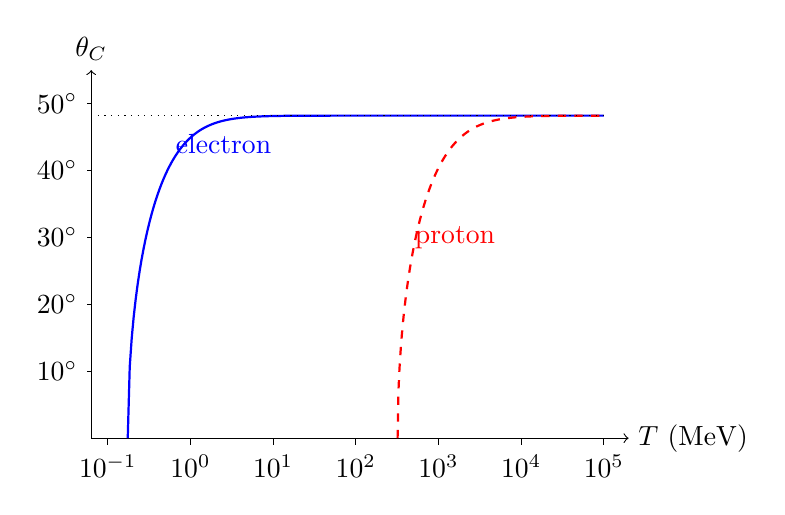
\begin{tikzpicture}[x=1.05cm,y=.085cm]
\draw[->] (-1.2,0)--(5.3,0) node[right] {$T\ (\mathrm{MeV})$};
\draw[->] (-1.2,0)--(-1.2,55) node[above] {$\theta_C$};
\draw (-1,0)--(-1,-1) node[below] {$10^{-1}$};
\draw (0,0)--(0,-1) node[below] {$10^{0}$};
\draw (1,0)--(1,-1) node[below] {$10^{1}$};
\draw (2,0)--(2,-1) node[below] {$10^{2}$};
\draw (3,0)--(3,-1) node[below] {$10^{3}$};
\draw (4,0)--(4,-1) node[below] {$10^{4}$};
\draw (5,0)--(5,-1) node[below] {$10^{5}$};
\draw (-1.2,10)--(-1.25,10) node[left] {$10^\circ$};
\draw (-1.2,20)--(-1.25,20) node[left] {$20^\circ$};
\draw (-1.2,30)--(-1.25,30) node[left] {$30^\circ$};
\draw (-1.2,40)--(-1.25,40) node[left] {$40^\circ$};
\draw (-1.2,50)--(-1.25,50) node[left] {$50^\circ$};
\draw[thick,blue] plot coordinates {(-0.758010,0.000457) (-0.733918,10.675712) (-0.709826,14.968223) (-0.685734,18.173589) (-0.661642,20.801835) (-0.637550,23.052365) (-0.613458,25.028379) (-0.589366,26.791753) (-0.565274,28.383188) (-0.541181,29.831244) (-0.517089,31.156935) (-0.492997,32.376308) (-0.468905,33.501983) (-0.444813,34.544129) (-0.420721,35.511107) (-0.396629,36.409917) (-0.372537,37.246505) (-0.348445,38.025990) (-0.324353,38.752832) (-0.300261,39.430957) (-0.276168,40.063855) (-0.252076,40.654654) (-0.227984,41.206178) (-0.203892,41.720996) (-0.179800,42.201458) (-0.155708,42.649727) (-0.131616,43.067803) (-0.107524,43.457543) (-0.083432,43.820679) (-0.059340,44.158830) (-0.035247,44.473516) (-0.011155,44.766167) (0.012937,45.038128) (0.037029,45.290673) (0.061121,45.525001) (0.085213,45.742250) (0.109305,45.943497) (0.133397,46.129760) (0.157489,46.302006) (0.181581,46.461148) (0.205673,46.608054) (0.229766,46.743542) (0.253858,46.868387) (0.277950,46.983323) (0.302042,47.089041) (0.326134,47.186195) (0.350226,47.275398) (0.374318,47.357230) (0.398410,47.432236) (0.422502,47.500925) (0.446594,47.563778) (0.470686,47.621242) (0.494779,47.673738) (0.518871,47.721656) (0.542963,47.765362) (0.567055,47.805197) (0.591147,47.841476) (0.615239,47.874494) (0.639331,47.904521) (0.663423,47.931812) (0.687515,47.956598) (0.711607,47.979096) (0.735700,47.999503) (0.759792,48.018004) (0.783884,48.034767) (0.807976,48.049947) (0.832068,48.063685) (0.856160,48.076113) (0.880252,48.087349) (0.904344,48.097504) (0.928436,48.106677) (0.952528,48.114959) (0.976620,48.122434) (1.000713,48.129178) (1.024805,48.135259) (1.048897,48.140742) (1.072989,48.145683) (1.097081,48.150133) (1.121173,48.154142) (1.145265,48.157750) (1.169357,48.160998) (1.193449,48.163921) (1.217541,48.166550) (1.241633,48.168914) (1.265726,48.171039) (1.289818,48.172950) (1.313910,48.174667) (1.338002,48.176210) (1.362094,48.177595) (1.386186,48.178840) (1.410278,48.179958) (1.434370,48.180961) (1.458462,48.181862) (1.482554,48.182671) (1.506646,48.183396) (1.530739,48.184047) (1.554831,48.184631) (1.578923,48.185155) (1.603015,48.185625) (1.627107,48.186047) (1.651199,48.186425) (1.675291,48.186764) (1.699383,48.187067) (1.723475,48.187340) (1.747567,48.187584) (1.771660,48.187803) (1.795752,48.187999) (1.819844,48.188175) (1.843936,48.188332) (1.868028,48.188473) (1.892120,48.188600) (1.916212,48.188713) (1.940304,48.188815) (1.964396,48.188905) (1.988488,48.188987) (2.012580,48.189060) (2.036673,48.189125) (2.060765,48.189184) (2.084857,48.189236) (2.108949,48.189283) (2.133041,48.189325) (2.157133,48.189363) (2.181225,48.189397) (2.205317,48.189427) (2.229409,48.189454) (2.253501,48.189478) (2.277593,48.189500) (2.301686,48.189519) (2.325778,48.189537) (2.349870,48.189552) (2.373962,48.189566) (2.398054,48.189579) (2.422146,48.189590) (2.446238,48.189600) (2.470330,48.189609) (2.494422,48.189617) (2.518514,48.189624) (2.542606,48.189630) (2.566699,48.189636) (2.590791,48.189641) (2.614883,48.189646) (2.638975,48.189650) (2.663067,48.189654) (2.687159,48.189657) (2.711251,48.189660) (2.735343,48.189663) (2.759435,48.189665) (2.783527,48.189667) (2.807620,48.189669) (2.831712,48.189671) (2.855804,48.189672) (2.879896,48.189673) (2.903988,48.189675) (2.928080,48.189676) (2.952172,48.189677) (2.976264,48.189678) (3.000356,48.189678) (3.024448,48.189679) (3.048540,48.189680) (3.072633,48.189680) (3.096725,48.189681) (3.120817,48.189681) (3.144909,48.189682) (3.169001,48.189682) (3.193093,48.189682) (3.217185,48.189683) (3.241277,48.189683) (3.265369,48.189683) (3.289461,48.189683) (3.313553,48.189684) (3.337646,48.189684) (3.361738,48.189684) (3.385830,48.189684) (3.409922,48.189684) (3.434014,48.189684) (3.458106,48.189684) (3.482198,48.189684) (3.506290,48.189684) (3.530382,48.189685) (3.554474,48.189685) (3.578567,48.189685) (3.602659,48.189685) (3.626751,48.189685) (3.650843,48.189685) (3.674935,48.189685) (3.699027,48.189685) (3.723119,48.189685) (3.747211,48.189685) (3.771303,48.189685) (3.795395,48.189685) (3.819487,48.189685) (3.843580,48.189685) (3.867672,48.189685) (3.891764,48.189685) (3.915856,48.189685) (3.939948,48.189685) (3.964040,48.189685) (3.988132,48.189685) (4.012224,48.189685) (4.036316,48.189685) (4.060408,48.189685) (4.084500,48.189685) (4.108593,48.189685) (4.132685,48.189685) (4.156777,48.189685) (4.180869,48.189685) (4.204961,48.189685) (4.229053,48.189685) (4.253145,48.189685) (4.277237,48.189685) (4.301329,48.189685) (4.325421,48.189685) (4.349513,48.189685) (4.373606,48.189685) (4.397698,48.189685) (4.421790,48.189685) (4.445882,48.189685) (4.469974,48.189685) (4.494066,48.189685) (4.518158,48.189685) (4.542250,48.189685) (4.566342,48.189685) (4.590434,48.189685) (4.614527,48.189685) (4.638619,48.189685) (4.662711,48.189685) (4.686803,48.189685) (4.710895,48.189685) (4.734987,48.189685) (4.759079,48.189685) (4.783171,48.189685) (4.807263,48.189685) (4.831355,48.189685) (4.855447,48.189685) (4.879540,48.189685) (4.903632,48.189685) (4.927724,48.189685) (4.951816,48.189685) (4.975908,48.189685) (5.000000,48.189685)};
\draw[thick,red,dashed] plot coordinates {(2.505899,0.000457) (2.516334,7.060306) (2.526770,9.947875) (2.537205,12.138399) (2.547641,13.964000) (2.558076,15.553840) (2.568512,16.974411) (2.578948,18.265362) (2.589383,19.452626) (2.599819,20.554280) (2.610254,21.583538) (2.620690,22.550412) (2.631125,23.462711) (2.641561,24.326669) (2.651997,25.147361) (2.662432,25.928986) (2.672868,26.675067) (2.683303,27.388599) (2.693739,28.072150) (2.704174,28.727948) (2.714610,29.357939) (2.725046,29.963837) (2.735481,30.547160) (2.745917,31.109263) (2.756352,31.651363) (2.766788,32.174553) (2.777223,32.679828) (2.787659,33.168090) (2.798095,33.640164) (2.808530,34.096805) (2.818966,34.538710) (2.829401,34.966522) (2.839837,35.380836) (2.850272,35.782203) (2.860708,36.171140) (2.871143,36.548126) (2.881579,36.913611) (2.892015,37.268017) (2.902450,37.611742) (2.912886,37.945159) (2.923321,38.268622) (2.933757,38.582464) (2.944192,38.887003) (2.954628,39.182538) (2.965064,39.469357) (2.975499,39.747730) (2.985935,40.017919) (2.996370,40.280170) (3.006806,40.534723) (3.017241,40.781803) (3.027677,41.021630) (3.038113,41.254413) (3.048548,41.480354) (3.058984,41.699646) (3.069419,41.912476) (3.079855,42.119025) (3.090290,42.319467) (3.100726,42.513969) (3.111162,42.702695) (3.121597,42.885803) (3.132033,43.063443) (3.142468,43.235766) (3.152904,43.402913) (3.163339,43.565025) (3.173775,43.722236) (3.184211,43.874678) (3.194646,44.022479) (3.205082,44.165764) (3.215517,44.304653) (3.225953,44.439265) (3.236388,44.569714) (3.246824,44.696112) (3.257260,44.818569) (3.267695,44.937190) (3.278131,45.052081) (3.288566,45.163341) (3.299002,45.271070) (3.309437,45.375365) (3.319873,45.476320) (3.330309,45.574026) (3.340744,45.668574) (3.351180,45.760051) (3.361615,45.848544) (3.372051,45.934135) (3.382486,46.016906) (3.392922,46.096938) (3.403358,46.174308) (3.413793,46.249093) (3.424229,46.321367) (3.434664,46.391202) (3.445100,46.458670) (3.455535,46.523841) (3.465971,46.586781) (3.476407,46.647557) (3.486842,46.706233) (3.497278,46.762873) (3.507713,46.817538) (3.518149,46.870287) (3.528584,46.921180) (3.539020,46.970274) (3.549456,47.017623) (3.559891,47.063283) (3.570327,47.107307) (3.580762,47.149745) (3.591198,47.190649) (3.601633,47.230066) (3.612069,47.268046) (3.622505,47.304634) (3.632940,47.339876) (3.643376,47.373816) (3.653811,47.406496) (3.664247,47.437958) (3.674682,47.468243) (3.685118,47.497391) (3.695554,47.525439) (3.705989,47.552425) (3.716425,47.578385) (3.726860,47.603354) (3.737296,47.627366) (3.747731,47.650456) (3.758167,47.672654) (3.768603,47.693992) (3.779038,47.714500) (3.789474,47.734208) (3.799909,47.753144) (3.810345,47.771337) (3.820780,47.788812) (3.831216,47.805595) (3.841652,47.821713) (3.852087,47.837188) (3.862523,47.852045) (3.872958,47.866307) (3.883394,47.879995) (3.893829,47.893132) (3.904265,47.905737) (3.914701,47.917830) (3.925136,47.929431) (3.935572,47.940559) (3.946007,47.951232) (3.956443,47.961466) (3.966878,47.971280) (3.977314,47.980688) (3.987750,47.989708) (3.998185,47.998353) (4.008621,48.006638) (4.019056,48.014578) (4.029492,48.022187) (4.039927,48.029476) (4.050363,48.036460) (4.060799,48.043149) (4.071234,48.049557) (4.081670,48.055693) (4.092105,48.061569) (4.102541,48.067196) (4.112976,48.072583) (4.123412,48.077741) (4.133848,48.082678) (4.144283,48.087404) (4.154719,48.091927) (4.165154,48.096255) (4.175590,48.100397) (4.186025,48.104361) (4.196461,48.108153) (4.206897,48.111780) (4.217332,48.115251) (4.227768,48.118570) (4.238203,48.121746) (4.248639,48.124782) (4.259074,48.127686) (4.269510,48.130463) (4.279946,48.133119) (4.290381,48.135658) (4.300817,48.138085) (4.311252,48.140405) (4.321688,48.142624) (4.332123,48.144744) (4.342559,48.146771) (4.352995,48.148708) (4.363430,48.150559) (4.373866,48.152328) (4.384301,48.154018) (4.394737,48.155634) (4.405172,48.157177) (4.415608,48.158652) (4.426044,48.160060) (4.436479,48.161406) (4.446915,48.162692) (4.457350,48.163920) (4.467786,48.165093) (4.478221,48.166213) (4.488657,48.167283) (4.499093,48.168305) (4.509528,48.169281) (4.519964,48.170213) (4.530399,48.171103) (4.540835,48.171953) (4.551270,48.172764) (4.561706,48.173539) (4.572142,48.174279) (4.582577,48.174985) (4.593013,48.175659) (4.603448,48.176303) (4.613884,48.176917) (4.624319,48.177503) (4.634755,48.178063) (4.645191,48.178598) (4.655626,48.179108) (4.666062,48.179594) (4.676497,48.180059) (4.686933,48.180502) (4.697368,48.180925) (4.707804,48.181329) (4.718240,48.181715) (4.728675,48.182082) (4.739111,48.182433) (4.749546,48.182768) (4.759982,48.183087) (4.770417,48.183392) (4.780853,48.183683) (4.791289,48.183961) (4.801724,48.184225) (4.812160,48.184478) (4.822595,48.184719) (4.833031,48.184949) (4.843466,48.185168) (4.853902,48.185378) (4.864338,48.185577) (4.874773,48.185768) (4.885209,48.185949) (4.895644,48.186123) (4.906080,48.186288) (4.916515,48.186445) (4.926951,48.186596) (4.937387,48.186739) (4.947822,48.186876) (4.958258,48.187007) (4.968693,48.187131) (4.979129,48.187250) (4.989564,48.187363) (5.000000,48.187471)};
\node[blue] at (0.4,44) {electron};
\node[red] at (3.2,30) {proton};
\draw[dotted] (-1.2,48.189685)--(5,48.189685);
\end{tikzpicture}

\end{center}
The horizontal energy axis is logarithmic; each curve starts at its own
threshold.

To count photons, divide the Frank--Tamm spectral energy (13.48) by
$\hbar\omega$:
\[
 \frac{d^2N_\gamma}{dx\,d\omega}
 =\frac{z^2e^2}{\hbar c^2}
  \left(1-\frac1{n^2\beta^2}\right).
\]
The specified wavelengths are vacuum wavelengths, so
$\omega=2\pi c/\lambda$ and
$|d\omega/d\lambda|=2\pi c/\lambda^2$. Thus
\[
 \frac{d^2N_\gamma}{dx\,d\lambda}
 =\frac{2\pi z^2\alpha}{\lambda^2}
  \left(1-\frac1{n^2\beta^2}\right),
\]
and for singly charged particles
\[
 \begin{split}
 \frac{N_\gamma}{x}
 &=2\pi\alpha
 \left(\frac1{4.000\times10^{-5}\ {\rm cm}}
      -\frac1{6.000\times10^{-5}\ {\rm cm}}\right)
 \left(1-\frac1{2.25\beta^2}\right)\\
 &=\boxed{382.088\left(1-\frac1{2.25\beta^2}\right){\rm cm^{-1}}.}
 \end{split}
\]
The resulting angles and yields are
\[
\begin{array}{c|rrr}
 \text{particle and kinetic energy}&\beta&\theta_C&
 N_\gamma/x\ ({\rm cm^{-1}})\\ \hline
 e,\ 1\ {\rm MeV}&0.94108&44.8946^\circ&190.34\\
 p,\ 500\ {\rm MeV}&0.75791&28.4042^\circ&86.46\\
 p,\ 5000\ {\rm MeV}&0.98744&47.5344^\circ&207.92
\end{array}
\]
These are emitted photon numbers. Absorption, interface escape losses,
and detector efficiency would be additional experimental factors.





\Needspace{5\baselineskip}
\par\bigskip
\noindent\textbf{13.10}\quad A particle of charge $ze$ moves along the $z$ axis with constant speed $v$, passing $z=0$ at $t=0$. The medium through which the particle moves is described by a dielectric constant $\epsilon(\omega)$.
\begin{enumerate}
\item[(a)] Beginning with the potential $\Phi(\mathbf{k},\omega)$ of (13.25), show that the potential of frequency $\omega$ is given as a function of spatial coordinate $\mathbf{x}$ by
\[
\Phi(\omega,\mathbf{x})=\frac{ze}{v\epsilon(\omega)}\sqrt{\frac{2}{\pi}}\;K_{0}\!\left(\frac{|\omega|\,\rho}{v}\sqrt{1-\beta^{2}\epsilon}\right)\!e^{i\omega z/v}
\]
where $z$ and $\rho=\sqrt{x^{2}+y^{2}}$ are the cylindrical coordinates of the observation point.
\item[(b)] Assuming that $\epsilon$ is independent of frequency and that $\beta^{2}\epsilon<1$, take the Fourier transform with respect to $\omega$ of the expression in part a and obtain $\Phi(\mathbf{x},t)$. Calculate the electric and magnetic fields and compare them to the vacuum fields (11.152). Show that, among other things, the vacuum factor $\gamma$ is replaced by $\Gamma=(1-\beta^{2}\epsilon)^{-1/2}$.
\item[(c)] Repeat the calculations of parts a and b with $\beta^{2}\epsilon>1$. Show that now
\[
\Phi(\omega,\mathbf{x})=\frac{ze}{v\epsilon(\omega)}\sqrt{\frac{\pi}{2}}\;e^{i\omega z/v}\!\left[-N_{0}\!\left(\frac{|\omega|\,\rho}{v}\sqrt{\beta^{2}\epsilon-1}\right)\pm iJ_{0}\!\left(\frac{|\omega|\,\rho}{v}\sqrt{\beta^{2}\epsilon-1}\right)\right]
\]
for $\omega\gtrless0$. Calculate the remaining Fourier transform to obtain $\Phi(\mathbf{x},t)$. Relate your answer to the result given in Section 13.4 for $\mathbf{A}(\mathbf{x},t)$.
\end{enumerate}
\solution
Write $q=ze$, let $\rho$ denote cylindrical radius, and assume a
nonmagnetic medium. The retarded prescription is essential, especially
above the Cherenkov threshold: take
$\operatorname{Im}\epsilon(\omega)>0$ for $\omega>0$ and then approach
the lossless limit.

\textbf{(a)} The symmetric four-dimensional transform in (13.25) is
\[
 \Phi(\mathbf k,\omega)
 =\frac{2q}{\epsilon(\omega)}
   \frac{\delta(\omega-vk_z)}
   {k_\perp^2+k_z^2-\epsilon(\omega)\omega^2/c^2}.
\]
Performing the $k_z$ integral in the three-dimensional inverse transform
gives
\[
 \Phi(\omega,\mathbf x)=
 \frac{2q\,e^{i\omega z/v}}{(2\pi)^{3/2}v\epsilon}
 \int\frac{d^2k_\perp\,e^{i\mathbf k_\perp\cdot\boldsymbol\rho}}
               {k_\perp^2+\lambda^2},
 \qquad
 \lambda^2=\frac{\omega^2}{v^2}(1-\beta^2\epsilon).
\]
The azimuthal integral is $2\pi J_0(k_\perp\rho)$. Initially take
$\lambda>0$ real, so that the auxiliary exponential integral converges.
A useful evaluation of the radial
integral is
\[
 \begin{split}
 \int_0^\infty\frac{kJ_0(k\rho)}{k^2+\lambda^2}\,dk
 &=\int_0^\infty e^{-s\lambda^2}ds
       \int_0^\infty kJ_0(k\rho)e^{-sk^2}\,dk\\
 &=\frac12\int_0^\infty\frac{ds}{s}
       e^{-s\lambda^2-\rho^2/(4s)}
 =K_0(\lambda\rho).
 \end{split}
\]
Analytic continuation to $\operatorname{Re}\lambda>0$ then implements
the retarded prescription. The intermediate real-$s$ representation
requires $\operatorname{Re}(\lambda^2)>0$; the continued Bessel
identity has the wider domain.
Combining the normalization factors gives
\[
 \boxed{\Phi(\omega,\mathbf x)
 =\frac{q}{v\epsilon(\omega)}\sqrt{\frac2\pi}\,
 K_0\!\left(\frac{|\omega|\rho}{v}
              \sqrt{1-\beta^2\epsilon(\omega)}\right)
 e^{i\omega z/v}.}
\]
The square-root branch is continued from positive real part, and the
negative-frequency potential is the complex conjugate of the
positive-frequency potential. Equation (13.25) also gives, at each
frequency, $\mathbf A=\beta\epsilon\Phi\,\hat{\mathbf z}$.

\textbf{(b)} Now let $\epsilon$ be a real positive constant and
$\beta^2\epsilon<1$. Define
\[
 \zeta=vt-z,\qquad
 \Gamma=(1-\beta^2\epsilon)^{-1/2},\qquad
 a=\frac{\rho}{\Gamma v},\qquad \tau=\frac{\zeta}{v}.
\]
Pairing positive and negative frequencies gives
\[
 \Phi(\mathbf x,t)=\frac{2q}{\pi v\epsilon}
       \int_0^\infty K_0(a\omega)\cos(\tau\omega)\,d\omega.
\]
For clarity, using $K_0(a\omega)=
\int_0^\infty e^{-a\omega\cosh u}du$ evaluates the integral as
\[
 \begin{split}
 \int_0^\infty K_0(a\omega)\cos(\tau\omega)d\omega
 &=\int_0^\infty
    \frac{a\cosh u}{a^2\cosh^2u+\tau^2}\,du\\
 &=a\int_0^\infty\frac{ds}{a^2s^2+a^2+\tau^2}
 =\frac{\pi}{2\sqrt{a^2+\tau^2}},
 \end{split}
\]
where $s=\sinh u$. Consequently
\[
 \boxed{\Phi(\mathbf x,t)
 =\frac{q}{\epsilon\sqrt{\zeta^2+\rho^2/\Gamma^2}}
 =\frac{q\Gamma}{\epsilon\sqrt{\rho^2+\Gamma^2\zeta^2}},
 \qquad A_z=\beta\epsilon\Phi.}
\]
Set $D=\rho^2+\Gamma^2\zeta^2$. Direct differentiation yields
\[
 E_\rho=-\partial_\rho\Phi
      =\frac{q\Gamma\rho}{\epsilon D^{3/2}}.
\]
For the longitudinal field, $\partial_z=-\partial_\zeta$ and
$\partial_t=v\partial_\zeta$, so both potentials contribute:
\[
 \begin{split}
 E_z&=-\partial_z\Phi-\frac1c\partial_tA_z
 =(1-\beta^2\epsilon)\partial_\zeta\Phi\\
 &=-\Gamma^{-2}\frac{q\Gamma^3\zeta}{\epsilon D^{3/2}}
 =-\frac{q\Gamma\zeta}{\epsilon D^{3/2}}.
 \end{split}
\]
Finally,
\[
 \boxed{\mathbf E=\frac{q\Gamma}
 {\epsilon[\rho^2+\Gamma^2(z-vt)^2]^{3/2}}
       [\rho\,\hat{\boldsymbol\rho}+(z-vt)\hat{\mathbf z}],
 \qquad
 \mathbf B=\beta\epsilon E_\rho\,\hat{\boldsymbol\phi}.}
\]
For $\epsilon=1$, $\Gamma=\gamma$, and these are precisely the
uniform-motion vacuum fields (11.152). In a medium the electric field
also carries a factor $1/\epsilon$, and the magnetic-to-transverse-electric
ratio becomes $\beta\epsilon$.

\textbf{(c)} Let $\kappa=\sqrt{\beta^2\epsilon-1}$ and now put
$a=\kappa\rho/v$. The retarded continuation gives
$\lambda\rho=-ia\omega$ for $\omega>0$. The Bessel continuation
\[
 K_0(-ix)=\frac{\pi}{2}[-N_0(x)+iJ_0(x)],\qquad x>0,
\]
and its complex conjugate for $\omega<0$ give
\[
 \boxed{\Phi(\omega,\mathbf x)=
 \frac{q}{v\epsilon}\sqrt{\frac\pi2}\,e^{i\omega z/v}
 [-N_0(a|\omega|)+i\,\operatorname{sgn}(\omega)J_0(a|\omega|)].}
\]
Here $N_0$ is Jackson's Neumann function. Pairing the two frequency
halves now yields
\[
 \Phi(\mathbf x,t)=\frac{q}{v\epsilon}
 \int_0^\infty[-N_0(a\omega)\cos(\tau\omega)
                    +J_0(a\omega)\sin(\tau\omega)]\,d\omega.
\]
These are retarded, regulated integrals. Their values follow by setting
$s=0^+-i\tau$ in the Laplace transforms
\[
 \int_0^\infty e^{-s\omega}J_0(a\omega)d\omega
   =\frac1{\sqrt{a^2+s^2}},\qquad
 \int_0^\infty e^{-s\omega}N_0(a\omega)d\omega
   =-\frac2\pi\frac{\operatorname{arsinh}(s/a)}
                     {\sqrt{a^2+s^2}}.
\]
Specifically,
\[
 \int_0^\infty J_0(a\omega)\sin(\tau\omega)d\omega
 =\frac{\operatorname{sgn}\tau\,H(|\tau|-a)}
       {\sqrt{\tau^2-a^2}},
 \qquad
 \int_0^\infty N_0(a\omega)\cos(\tau\omega)d\omega
 =-\frac{H(|\tau|-a)}{\sqrt{\tau^2-a^2}}.
\]
They cancel for $\tau<-a$, both have zero relevant part for $|\tau|<a$,
and add for $\tau>a$. Thus
\[
 \boxed{\Phi(\mathbf x,t)=
 \frac{2q}{\epsilon}
 \frac{H(\zeta-\kappa\rho)}{\sqrt{\zeta^2-\kappa^2\rho^2}},
 \qquad
 \mathbf A=\frac{2q\beta\,H(\zeta-\kappa\rho)}
                 {\sqrt{\zeta^2-\kappa^2\rho^2}}\hat{\mathbf z}.}
\]
The vector potential agrees with (13.51), after rotating Jackson's
direction of motion from $x$ to $z$. It is nonzero only inside the
wake behind the particle. The factor of two reflects the two retarded
source positions contributing inside a superluminal cone.

For points strictly inside the cone, put $S=\zeta^2-\kappa^2\rho^2$.
The regular parts of the fields are
\[
 \boxed{E_\rho=-\frac{2q\kappa^2\rho}{\epsilon S^{3/2}},
 \qquad E_z=\frac{2q\kappa^2\zeta}{\epsilon S^{3/2}},
 \qquad B_\phi=\beta\epsilon E_\rho.}
\]
They vanish strictly outside the cone. At the front one must
differentiate the whole regulated potential, including its support,
before removing the regulator; the divergent front is not represented
by these interior formulas alone. The assumption of a frequency-independent
dielectric constant creates this singularity, as discussed immediately
after (13.51). Dispersion and absorption regularize a physical front.





\Needspace{5\baselineskip}
\par\bigskip
\noindent\textbf{13.11}\quad A magnetic monopole with magnetic charge $g$ passes through matter and loses energy by collisions with electrons, just as does a particle with electric charge $ze$.
\begin{enumerate}
\item[(a)] In the same approximation as presented in Section 13.1, show that the energy loss per unit distance is given approximately by (13.14), but with $ze\to\beta g$ \erratum{and with only the leading logarithm retained}, yielding
\[
\left(\frac{dE}{dx}\right)_{\substack{\mathrm{magnetic}\\ \mathrm{monopole}}}\simeq4\pi NZ\,\frac{g^{2}e^{2}}{mc^{2}}\ln\!\left(\frac{2\gamma^{2}mv^{2}}{\hbar\langle\omega\rangle}\right)
\]
\item[(b)] With the Dirac quantization condition (6.153) determining the magnetic charge, what $z$ value is necessary for an ordinary charged particle in order that it lose energy at relativistic speeds at the same rate as a monopole? Sketch for the magnetic monopole a curve of $dE/dx$ equivalent to Fig.~13.1 and comment on the differences.
\end{enumerate}
\solution
\textbf{(a)} In Gaussian units the static monopole field is
$\mathbf B'=g\mathbf r'/r'^3$. A boost along its path gives
\[
 B_\perp(t)=\frac{g\gamma b}{(b^2+\gamma^2v^2t^2)^{3/2}},
 \qquad \mathbf E=-\boldsymbol\beta\times\mathbf B.
\]
An initially slow electron is accelerated by this transverse electric
field. Its magnitude is exactly the electric-charge expression of
Problem 13.1(b) with $ze$ replaced by $\beta g$, although its direction
is rotated by $90^\circ$ around the trajectory. Thus
\[
 |\Delta p|=\frac{2e\beta g}{bv}
           =\frac{2eg}{bc},\qquad
 \Delta E(b)=\frac{2e^2g^2}{mc^2b^2}.
\]
For electron density $n_e=NZ$, integrating over impact parameters gives
\[
 S_g=2\pi n_e\int b\,\Delta E(b)\,db
 =\frac{4\pi NZg^2e^2}{mc^2}\ln\frac{b_{\max}}{b_{\min}}.
\]
The bound-electron and quantum matching used in Section 13.1 sets
the logarithm to $\ln B_q$, with
$B_q=2\gamma^2mv^2/(\hbar\langle\omega\rangle)$, to the accuracy
retained here. Therefore
\[
 \boxed{S_g\simeq\frac{4\pi NZg^2e^2}{mc^2}
 \ln\frac{2\gamma^2mv^2}{\hbar\langle\omega\rangle}.}
\]
There is no $1/\beta^2$ prefactor: the extra $\beta$ in the induced
electric field cancels it.

The displayed result is a \emph{leading-logarithm} formula.
A literal algebraic substitution in the full electric-charge (13.14)
would leave $\ln B_q-\beta^2$ rather than $\ln B_q$.
The omitted nonlogarithmic term, and monopole-specific corrections
beyond this impulse treatment, cannot be inferred from the replacement
rule. The marked qualification in the statement makes the approximation
consistent.

\textbf{(b)} Converting the Dirac condition (6.153) to the Gaussian
normalization used here gives
\[
 eg=\frac{n\hbar c}{2},\qquad
 \frac ge=\frac{n}{2\alpha}.
\]
Since $\beta\simeq1$ at relativistic speed, the equivalent ordinary
charge is
\[
 \boxed{z_{\rm equivalent}\simeq\frac{|g|}{e}
       =68.518\,|n|.}
\]
For the minimum monopole, the stopping power at such speeds is therefore
roughly $(68.518)^2\simeq4695$ times that of a singly charged particle,
at the same leading-logarithm accuracy.

To compare shapes with Fig.~13.1, put $u=\gamma\beta$ and use the
figure's $I=160$ eV. Divide out the squared effective charge:
\[
 S_{\rm plot,g}=0.15\ln\frac{2mc^2u^2}{I},\qquad
 S_{\rm plot,e}=\frac{0.15}{\beta^2}
       \left[\ln\frac{2mc^2u^2}{I}-\beta^2\right],
 \qquad \beta^2=\frac{u^2}{1+u^2}.
\]
The resulting sketch uses logarithmic axes:
\begin{center}
% Generated by supplementary/check_ch13.py --figures
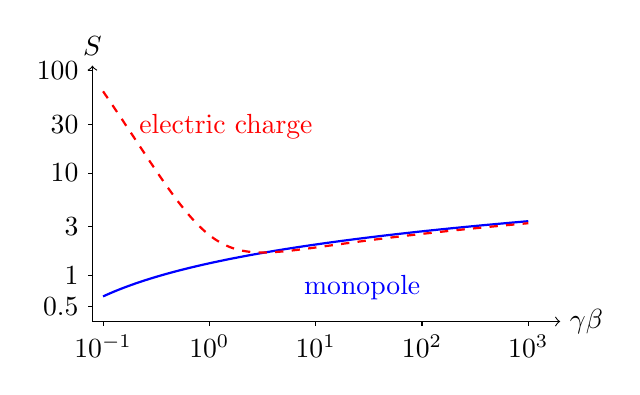
\begin{tikzpicture}[x=1.35cm,y=1.3cm]
\draw[->] (-1.1,-.45)--(3.3,-.45) node[right] {$\gamma\beta$};
\draw[->] (-1.1,-.45)--(-1.1,2.05) node[above] {$S$};
\draw (-1,-.45)--(-1,-.49) node[below] {$10^{-1}$};
\draw (0,-.45)--(0,-.49) node[below] {$10^{0}$};
\draw (1,-.45)--(1,-.49) node[below] {$10^{1}$};
\draw (2,-.45)--(2,-.49) node[below] {$10^{2}$};
\draw (3,-.45)--(3,-.49) node[below] {$10^{3}$};
\draw (-1.1,-0.3010299956639812)--(-1.14,-0.3010299956639812) node[left] {$0.5$};
\draw (-1.1,0.0)--(-1.14,0.0) node[left] {$1$};
\draw (-1.1,0.47712125471966244)--(-1.14,0.47712125471966244) node[left] {$3$};
\draw (-1.1,1.0)--(-1.14,1.0) node[left] {$10$};
\draw (-1.1,1.4771212547196624)--(-1.14,1.4771212547196624) node[left] {$30$};
\draw (-1.1,2.0)--(-1.14,2.0) node[left] {$100$};
\draw[blue,thick] plot coordinates {(-1.000000,-0.205136) (-0.988539,-0.199657) (-0.977077,-0.194246) (-0.965616,-0.188901) (-0.954155,-0.183621) (-0.942693,-0.178405) (-0.931232,-0.173250) (-0.919771,-0.168156) (-0.908309,-0.163121) (-0.896848,-0.158144) (-0.885387,-0.153223) (-0.873926,-0.148358) (-0.862464,-0.143546) (-0.851003,-0.138787) (-0.839542,-0.134079) (-0.828080,-0.129422) (-0.816619,-0.124815) (-0.805158,-0.120256) (-0.793696,-0.115744) (-0.782235,-0.111278) (-0.770774,-0.106858) (-0.759312,-0.102483) (-0.747851,-0.098151) (-0.736390,-0.093862) (-0.724928,-0.089615) (-0.713467,-0.085409) (-0.702006,-0.081243) (-0.690544,-0.077117) (-0.679083,-0.073030) (-0.667622,-0.068981) (-0.656160,-0.064969) (-0.644699,-0.060994) (-0.633238,-0.057055) (-0.621777,-0.053152) (-0.610315,-0.049283) (-0.598854,-0.045448) (-0.587393,-0.041647) (-0.575931,-0.037879) (-0.564470,-0.034144) (-0.553009,-0.030440) (-0.541547,-0.026767) (-0.530086,-0.023126) (-0.518625,-0.019514) (-0.507163,-0.015933) (-0.495702,-0.012380) (-0.484241,-0.008857) (-0.472779,-0.005362) (-0.461318,-0.001895) (-0.449857,0.001545) (-0.438395,0.004958) (-0.426934,0.008344) (-0.415473,0.011704) (-0.404011,0.015038) (-0.392550,0.018347) (-0.381089,0.021631) (-0.369628,0.024890) (-0.358166,0.028125) (-0.346705,0.031335) (-0.335244,0.034523) (-0.323782,0.037687) (-0.312321,0.040828) (-0.300860,0.043947) (-0.289398,0.047043) (-0.277937,0.050118) (-0.266476,0.053171) (-0.255014,0.056202) (-0.243553,0.059213) (-0.232092,0.062202) (-0.220630,0.065172) (-0.209169,0.068121) (-0.197708,0.071050) (-0.186246,0.073960) (-0.174785,0.076850) (-0.163324,0.079722) (-0.151862,0.082574) (-0.140401,0.085408) (-0.128940,0.088223) (-0.117479,0.091021) (-0.106017,0.093800) (-0.094556,0.096562) (-0.083095,0.099306) (-0.071633,0.102033) (-0.060172,0.104743) (-0.048711,0.107436) (-0.037249,0.110113) (-0.025788,0.112773) (-0.014327,0.115417) (-0.002865,0.118045) (0.008596,0.120657) (0.020057,0.123254) (0.031519,0.125835) (0.042980,0.128401) (0.054441,0.130951) (0.065903,0.133487) (0.077364,0.136008) (0.088825,0.138515) (0.100287,0.141007) (0.111748,0.143485) (0.123209,0.145949) (0.134670,0.148399) (0.146132,0.150836) (0.157593,0.153259) (0.169054,0.155668) (0.180516,0.158064) (0.191977,0.160447) (0.203438,0.162817) (0.214900,0.165174) (0.226361,0.167518) (0.237822,0.169850) (0.249284,0.172169) (0.260745,0.174476) (0.272206,0.176771) (0.283668,0.179053) (0.295129,0.181324) (0.306590,0.183583) (0.318052,0.185830) (0.329513,0.188066) (0.340974,0.190290) (0.352436,0.192503) (0.363897,0.194705) (0.375358,0.196895) (0.386819,0.199075) (0.398281,0.201243) (0.409742,0.203401) (0.421203,0.205548) (0.432665,0.207685) (0.444126,0.209811) (0.455587,0.211927) (0.467049,0.214033) (0.478510,0.216128) (0.489971,0.218214) (0.501433,0.220289) (0.512894,0.222355) (0.524355,0.224410) (0.535817,0.226456) (0.547278,0.228493) (0.558739,0.230520) (0.570201,0.232537) (0.581662,0.234546) (0.593123,0.236545) (0.604585,0.238535) (0.616046,0.240515) (0.627507,0.242487) (0.638968,0.244450) (0.650430,0.246404) (0.661891,0.248349) (0.673352,0.250286) (0.684814,0.252214) (0.696275,0.254133) (0.707736,0.256044) (0.719198,0.257947) (0.730659,0.259841) (0.742120,0.261727) (0.753582,0.263605) (0.765043,0.265475) (0.776504,0.267337) (0.787966,0.269191) (0.799427,0.271037) (0.810888,0.272875) (0.822350,0.274706) (0.833811,0.276529) (0.845272,0.278344) (0.856734,0.280151) (0.868195,0.281952) (0.879656,0.283744) (0.891117,0.285530) (0.902579,0.287308) (0.914040,0.289078) (0.925501,0.290842) (0.936963,0.292598) (0.948424,0.294348) (0.959885,0.296090) (0.971347,0.297825) (0.982808,0.299554) (0.994269,0.301276) (1.005731,0.302990) (1.017192,0.304699) (1.028653,0.306400) (1.040115,0.308095) (1.051576,0.309783) (1.063037,0.311464) (1.074499,0.313140) (1.085960,0.314808) (1.097421,0.316471) (1.108883,0.318127) (1.120344,0.319776) (1.131805,0.321420) (1.143266,0.323057) (1.154728,0.324688) (1.166189,0.326313) (1.177650,0.327932) (1.189112,0.329545) (1.200573,0.331152) (1.212034,0.332753) (1.223496,0.334348) (1.234957,0.335938) (1.246418,0.337521) (1.257880,0.339099) (1.269341,0.340671) (1.280802,0.342237) (1.292264,0.343798) (1.303725,0.345353) (1.315186,0.346903) (1.326648,0.348447) (1.338109,0.349986) (1.349570,0.351519) (1.361032,0.353047) (1.372493,0.354569) (1.383954,0.356086) (1.395415,0.357598) (1.406877,0.359105) (1.418338,0.360606) (1.429799,0.362102) (1.441261,0.363594) (1.452722,0.365080) (1.464183,0.366561) (1.475645,0.368036) (1.487106,0.369507) (1.498567,0.370973) (1.510029,0.372434) (1.521490,0.373890) (1.532951,0.375342) (1.544413,0.376788) (1.555874,0.378230) (1.567335,0.379666) (1.578797,0.381099) (1.590258,0.382526) (1.601719,0.383949) (1.613181,0.385367) (1.624642,0.386780) (1.636103,0.388189) (1.647564,0.389593) (1.659026,0.390993) (1.670487,0.392388) (1.681948,0.393779) (1.693410,0.395166) (1.704871,0.396548) (1.716332,0.397925) (1.727794,0.399298) (1.739255,0.400667) (1.750716,0.402032) (1.762178,0.403392) (1.773639,0.404748) (1.785100,0.406100) (1.796562,0.407448) (1.808023,0.408791) (1.819484,0.410131) (1.830946,0.411466) (1.842407,0.412797) (1.853868,0.414124) (1.865330,0.415447) (1.876791,0.416766) (1.888252,0.418081) (1.899713,0.419392) (1.911175,0.420699) (1.922636,0.422003) (1.934097,0.423302) (1.945559,0.424597) (1.957020,0.425889) (1.968481,0.427177) (1.979943,0.428460) (1.991404,0.429741) (2.002865,0.431017) (2.014327,0.432290) (2.025788,0.433559) (2.037249,0.434824) (2.048711,0.436085) (2.060172,0.437343) (2.071633,0.438597) (2.083095,0.439848) (2.094556,0.441095) (2.106017,0.442339) (2.117479,0.443579) (2.128940,0.444815) (2.140401,0.446048) (2.151862,0.447277) (2.163324,0.448503) (2.174785,0.449726) (2.186246,0.450945) (2.197708,0.452160) (2.209169,0.453373) (2.220630,0.454581) (2.232092,0.455787) (2.243553,0.456989) (2.255014,0.458188) (2.266476,0.459383) (2.277937,0.460576) (2.289398,0.461765) (2.300860,0.462951) (2.312321,0.464133) (2.323782,0.465312) (2.335244,0.466489) (2.346705,0.467661) (2.358166,0.468831) (2.369628,0.469998) (2.381089,0.471161) (2.392550,0.472322) (2.404011,0.473479) (2.415473,0.474633) (2.426934,0.475785) (2.438395,0.476933) (2.449857,0.478078) (2.461318,0.479220) (2.472779,0.480359) (2.484241,0.481495) (2.495702,0.482628) (2.507163,0.483759) (2.518625,0.484886) (2.530086,0.486010) (2.541547,0.487132) (2.553009,0.488250) (2.564470,0.489366) (2.575931,0.490479) (2.587393,0.491589) (2.598854,0.492696) (2.610315,0.493800) (2.621777,0.494902) (2.633238,0.496001) (2.644699,0.497097) (2.656160,0.498190) (2.667622,0.499280) (2.679083,0.500368) (2.690544,0.501453) (2.702006,0.502536) (2.713467,0.503615) (2.724928,0.504692) (2.736390,0.505766) (2.747851,0.506838) (2.759312,0.507907) (2.770774,0.508973) (2.782235,0.510037) (2.793696,0.511098) (2.805158,0.512157) (2.816619,0.513213) (2.828080,0.514267) (2.839542,0.515317) (2.851003,0.516366) (2.862464,0.517412) (2.873926,0.518455) (2.885387,0.519496) (2.896848,0.520534) (2.908309,0.521570) (2.919771,0.522603) (2.931232,0.523634) (2.942693,0.524663) (2.954155,0.525689) (2.965616,0.526713) (2.977077,0.527734) (2.988539,0.528753) (3.000000,0.529769)};
\draw[red,dashed,thick] plot coordinates {(-1.000000,1.798149) (-0.988539,1.780897) (-0.977077,1.763588) (-0.965616,1.746223) (-0.954155,1.728805) (-0.942693,1.711336) (-0.931232,1.693818) (-0.919771,1.676254) (-0.908309,1.658645) (-0.896848,1.640994) (-0.885387,1.623303) (-0.873926,1.605574) (-0.862464,1.587809) (-0.851003,1.570010) (-0.839542,1.552180) (-0.828080,1.534320) (-0.816619,1.516433) (-0.805158,1.498522) (-0.793696,1.480587) (-0.782235,1.462633) (-0.770774,1.444660) (-0.759312,1.426671) (-0.747851,1.408670) (-0.736390,1.390657) (-0.724928,1.372636) (-0.713467,1.354609) (-0.702006,1.336579) (-0.690544,1.318548) (-0.679083,1.300520) (-0.667622,1.282496) (-0.656160,1.264481) (-0.644699,1.246477) (-0.633238,1.228487) (-0.621777,1.210514) (-0.610315,1.192561) (-0.598854,1.174632) (-0.587393,1.156731) (-0.575931,1.138860) (-0.564470,1.121024) (-0.553009,1.103227) (-0.541547,1.085472) (-0.530086,1.067763) (-0.518625,1.050104) (-0.507163,1.032501) (-0.495702,1.014956) (-0.484241,0.997475) (-0.472779,0.980063) (-0.461318,0.962724) (-0.449857,0.945464) (-0.438395,0.928287) (-0.426934,0.911198) (-0.415473,0.894203) (-0.404011,0.877308) (-0.392550,0.860518) (-0.381089,0.843839) (-0.369628,0.827277) (-0.358166,0.810837) (-0.346705,0.794526) (-0.335244,0.778351) (-0.323782,0.762317) (-0.312321,0.746431) (-0.300860,0.730699) (-0.289398,0.715128) (-0.277937,0.699725) (-0.266476,0.684496) (-0.255014,0.669447) (-0.243553,0.654586) (-0.232092,0.639920) (-0.220630,0.625454) (-0.209169,0.611195) (-0.197708,0.597150) (-0.186246,0.583326) (-0.174785,0.569727) (-0.163324,0.556362) (-0.151862,0.543235) (-0.140401,0.530352) (-0.128940,0.517719) (-0.117479,0.505342) (-0.106017,0.493225) (-0.094556,0.481373) (-0.083095,0.469790) (-0.071633,0.458482) (-0.060172,0.447451) (-0.048711,0.436701) (-0.037249,0.426235) (-0.025788,0.416056) (-0.014327,0.406165) (-0.002865,0.396566) (0.008596,0.387258) (0.020057,0.378244) (0.031519,0.369524) (0.042980,0.361097) (0.054441,0.352963) (0.065903,0.345123) (0.077364,0.337573) (0.088825,0.330313) (0.100287,0.323340) (0.111748,0.316652) (0.123209,0.310246) (0.134670,0.304119) (0.146132,0.298267) (0.157593,0.292686) (0.169054,0.287372) (0.180516,0.282321) (0.191977,0.277527) (0.203438,0.272985) (0.214900,0.268690) (0.226361,0.264637) (0.237822,0.260820) (0.249284,0.257233) (0.260745,0.253870) (0.272206,0.250725) (0.283668,0.247792) (0.295129,0.245064) (0.306590,0.242536) (0.318052,0.240201) (0.329513,0.238054) (0.340974,0.236086) (0.352436,0.234294) (0.363897,0.232670) (0.375358,0.231208) (0.386819,0.229902) (0.398281,0.228746) (0.409742,0.227735) (0.421203,0.226863) (0.432665,0.226124) (0.444126,0.225513) (0.455587,0.225024) (0.467049,0.224652) (0.478510,0.224392) (0.489971,0.224239) (0.501433,0.224188) (0.512894,0.224235) (0.524355,0.224375) (0.535817,0.224604) (0.547278,0.224918) (0.558739,0.225311) (0.570201,0.225782) (0.581662,0.226325) (0.593123,0.226937) (0.604585,0.227615) (0.616046,0.228355) (0.627507,0.229154) (0.638968,0.230009) (0.650430,0.230916) (0.661891,0.231874) (0.673352,0.232879) (0.684814,0.233929) (0.696275,0.235021) (0.707736,0.236153) (0.719198,0.237322) (0.730659,0.238527) (0.742120,0.239765) (0.753582,0.241034) (0.765043,0.242333) (0.776504,0.243659) (0.787966,0.245011) (0.799427,0.246387) (0.810888,0.247786) (0.822350,0.249206) (0.833811,0.250646) (0.845272,0.252104) (0.856734,0.253579) (0.868195,0.255070) (0.879656,0.256576) (0.891117,0.258096) (0.902579,0.259628) (0.914040,0.261172) (0.925501,0.262726) (0.936963,0.264291) (0.948424,0.265864) (0.959885,0.267445) (0.971347,0.269034) (0.982808,0.270630) (0.994269,0.272231) (1.005731,0.273838) (1.017192,0.275450) (1.028653,0.277065) (1.040115,0.278685) (1.051576,0.280307) (1.063037,0.281933) (1.074499,0.283560) (1.085960,0.285189) (1.097421,0.286820) (1.108883,0.288451) (1.120344,0.290083) (1.131805,0.291715) (1.143266,0.293348) (1.154728,0.294979) (1.166189,0.296610) (1.177650,0.298241) (1.189112,0.299870) (1.200573,0.301497) (1.212034,0.303123) (1.223496,0.304747) (1.234957,0.306369) (1.246418,0.307988) (1.257880,0.309606) (1.269341,0.311220) (1.280802,0.312832) (1.292264,0.314441) (1.303725,0.316047) (1.315186,0.317650) (1.326648,0.319249) (1.338109,0.320845) (1.349570,0.322438) (1.361032,0.324027) (1.372493,0.325612) (1.383954,0.327193) (1.395415,0.328771) (1.406877,0.330345) (1.418338,0.331915) (1.429799,0.333481) (1.441261,0.335042) (1.452722,0.336600) (1.464183,0.338153) (1.475645,0.339703) (1.487106,0.341248) (1.498567,0.342788) (1.510029,0.344325) (1.521490,0.345857) (1.532951,0.347384) (1.544413,0.348908) (1.555874,0.350427) (1.567335,0.351941) (1.578797,0.353451) (1.590258,0.354957) (1.601719,0.356458) (1.613181,0.357954) (1.624642,0.359446) (1.636103,0.360934) (1.647564,0.362417) (1.659026,0.363896) (1.670487,0.365370) (1.681948,0.366840) (1.693410,0.368305) (1.704871,0.369766) (1.716332,0.371223) (1.727794,0.372675) (1.739255,0.374122) (1.750716,0.375565) (1.762178,0.377004) (1.773639,0.378438) (1.785100,0.379868) (1.796562,0.381293) (1.808023,0.382714) (1.819484,0.384131) (1.830946,0.385543) (1.842407,0.386951) (1.853868,0.388355) (1.865330,0.389755) (1.876791,0.391150) (1.888252,0.392541) (1.899713,0.393927) (1.911175,0.395310) (1.922636,0.396688) (1.934097,0.398062) (1.945559,0.399431) (1.957020,0.400797) (1.968481,0.402159) (1.979943,0.403516) (1.991404,0.404869) (2.002865,0.406218) (2.014327,0.407563) (2.025788,0.408904) (2.037249,0.410242) (2.048711,0.411575) (2.060172,0.412904) (2.071633,0.414229) (2.083095,0.415550) (2.094556,0.416867) (2.106017,0.418180) (2.117479,0.419490) (2.128940,0.420795) (2.140401,0.422097) (2.151862,0.423395) (2.163324,0.424689) (2.174785,0.425979) (2.186246,0.427265) (2.197708,0.428548) (2.209169,0.429827) (2.220630,0.431102) (2.232092,0.432374) (2.243553,0.433642) (2.255014,0.434906) (2.266476,0.436167) (2.277937,0.437424) (2.289398,0.438677) (2.300860,0.439927) (2.312321,0.441173) (2.323782,0.442416) (2.335244,0.443655) (2.346705,0.444891) (2.358166,0.446123) (2.369628,0.447352) (2.381089,0.448577) (2.392550,0.449799) (2.404011,0.451017) (2.415473,0.452232) (2.426934,0.453444) (2.438395,0.454653) (2.449857,0.455858) (2.461318,0.457059) (2.472779,0.458258) (2.484241,0.459453) (2.495702,0.460645) (2.507163,0.461833) (2.518625,0.463019) (2.530086,0.464201) (2.541547,0.465380) (2.553009,0.466555) (2.564470,0.467728) (2.575931,0.468897) (2.587393,0.470064) (2.598854,0.471227) (2.610315,0.472387) (2.621777,0.473544) (2.633238,0.474698) (2.644699,0.475849) (2.656160,0.476997) (2.667622,0.478142) (2.679083,0.479283) (2.690544,0.480422) (2.702006,0.481558) (2.713467,0.482691) (2.724928,0.483821) (2.736390,0.484948) (2.747851,0.486072) (2.759312,0.487193) (2.770774,0.488312) (2.782235,0.489427) (2.793696,0.490540) (2.805158,0.491650) (2.816619,0.492757) (2.828080,0.493861) (2.839542,0.494962) (2.851003,0.496061) (2.862464,0.497157) (2.873926,0.498250) (2.885387,0.499340) (2.896848,0.500427) (2.908309,0.501512) (2.919771,0.502594) (2.931232,0.503674) (2.942693,0.504751) (2.954155,0.505825) (2.965616,0.506896) (2.977077,0.507965) (2.988539,0.509031) (3.000000,0.510095)};
\node[blue,anchor=west] at (.8,-.12) {monopole};
\node[red,anchor=west] at (-.75,1.45) {electric charge};
\end{tikzpicture}

\end{center}
Its ordinate $S$ is the same approximate aluminum scale as Fig.~13.1,
after dividing the physical stopping power by $(g/e)^2$ for the
monopole or by $z^2$ for the electric particle. The monopole curve
rises logarithmically with $u$, whereas the electric curve has a
large low-speed rise and a minimum. Both rise logarithmically at
large $u$. In particular, the monopole lacks the electric particle's
$1/\beta^2$ increase near the end of its range. Neither this
high-speed approximation nor a negative extrapolation of its logarithm
describes the actual stopping law arbitrarily close to rest.





\Needspace{5\baselineskip}
\par\bigskip
\noindent\textbf{13.12}\quad A relativistic particle of charge $ze$ moves along the $z$ axis with a constant speed $\beta c$. The half-space $z\leq0$ is filled with a uniform isotropic dielectric medium with plasma frequency $\omega_{1}$, and the space $z>0$ with a similar medium whose plasma frequency is $\omega_{2}$. Discuss the emission of transition radiation as the particle traverses the interface, using the approximation of Section 13.7.
\begin{enumerate}
\item[(a)] Show that the radiation intensity per unit circular frequency interval and per unit solid angle is given approximately by
\[
\frac{d^{2}I}{d\omega\;d\Omega}\simeq\frac{z^{2}e^{2}\theta^{2}}{\pi^{2}c}\;
\left|\frac{1}{\dfrac{1}{\gamma^{2}}+\dfrac{\omega_{1}^{2}}{\omega^{2}}+\theta^{2}}
-\frac{1}{\dfrac{1}{\gamma^{2}}+\dfrac{\omega_{2}^{2}}{\omega^{2}}+\theta^{2}}\right|^{2}
\]
where $\theta$ is the angle of emission relative to the velocity of the particle and $\gamma=(1-\beta^{2})^{-1/2}$.
\item[(b)] Show that the total energy radiated is
\[
I\simeq\frac{z^{2}e^{2}}{3c}\cdot\frac{(\omega_{1}-\omega_{2})^{2}}{(\omega_{1}+\omega_{2})}\cdot\gamma
\]
\end{enumerate}
\solution
\textbf{(a)} Adopt the assumptions of Section 13.7:
$\gamma\gg1$, $\theta\ll1$, $\omega\gg\omega_j$, negligible absorption
and reflection, and
$\epsilon_j=1-\omega_j^2/\omega^2$. Define
\[
 A=\gamma^{-2}+\theta^2,\qquad
 q_j=\frac{\omega}{v}-k_j\cos\theta
 \simeq\frac{\omega}{2c}
       \left(A+\frac{\omega_j^2}{\omega^2}\right).
\]
The polarization driving the radiation is proportional to
$\omega_j^2\mathbf E_i$, while its longitudinal phase is $e^{iq_jz}$.
With convergence factors at infinity the two half-space integrals have
opposite signs:
\[
 \int_{-\infty}^0e^{iq_1z+0^+z}dz=\frac1{iq_1},
 \qquad
 \int_0^\infty e^{iq_2z-0^+z}dz=-\frac1{iq_2}.
\]
The transverse integral and its normalization can be kept explicit.
Write $q=ze$, $\ell=\omega/(\gamma v)$, $h=k\sin\theta$, and
$C=\sqrt{2/\pi}\,q\omega/(\gamma v^2)$. The incident fields are
$E_\rho=CK_1(\ell\rho)$ and $E_z=-iCK_0(\ell\rho)/\gamma$
after removing their common $z$ phase. The two-dimensional transform
and its derivative give
\[
\int d^2\rho\,e^{-ihx}K_0(\ell\rho)=\frac{2\pi}{\ell^2+h^2},
\qquad
\int d^2\rho\,e^{-ihx}\cos\phi K_1(\ell\rho)
=-\frac{2\pi i h}{\ell(\ell^2+h^2)}.
\]
For the second identity use
$\cos\phi K_1(\ell\rho)=-\ell^{-1}\partial_xK_0(\ell\rho)$
and integrate by parts. Projection onto the radiation polarization
in the observation plane gives
\[
T=\cos\theta\,T_\rho-\sin\theta\,T_z
=-\frac{2\pi i C}{\ell^2+h^2}
 \left(\frac{h\cos\theta}{\ell}-\frac{\sin\theta}{\gamma}\right)
\simeq-\frac{2i\sqrt{2\pi}\,q}{\omega}\frac{\theta}{A}.
\]
Here $v\simeq c$, $h\simeq\omega\theta/c$, and the retained denominator
is $\ell^2+h^2\simeq(\omega^2/c^2)A$.
Generalizing (13.79) to the two media therefore gives
\[
\frac{d^2I}{d\omega\,d\Omega}
=\frac1{32\pi^3c^3}
 \left|T\left(\frac{\omega_1^2}{iq_1}
                   -\frac{\omega_2^2}{iq_2}\right)\right|^2.
\]
Inserting $q_j$ leaves a common amplitude factor
$4\sqrt{2\pi}\,qc$ multiplying
\[
 \begin{split}
 \frac{\theta}{A}
 \left[\frac{\omega_2^2}{A\omega^2+\omega_2^2}
       -\frac{\omega_1^2}{A\omega^2+\omega_1^2}\right]
 &=\frac{\theta}{A}
 \left[\left(1-\frac{A\omega^2}{A\omega^2+\omega_2^2}\right)
       -\left(1-\frac{A\omega^2}{A\omega^2+\omega_1^2}\right)\right]\\
 &=\theta\left[
 \frac1{A+\omega_1^2/\omega^2}
 -\frac1{A+\omega_2^2/\omega^2}\right].
 \end{split}
\]
Squaring and using
$(4\sqrt{2\pi}\,qc)^2/(32\pi^3c^3)=q^2/(\pi^2c)$ gives
\[
 \boxed{\frac{d^2I}{d\omega\,d\Omega}
 =\frac{z^2e^2\theta^2}{\pi^2c}
 \left|\frac1{\gamma^{-2}+\theta^2+\omega_1^2/\omega^2}
       -\frac1{\gamma^{-2}+\theta^2+\omega_2^2/\omega^2}\right|^2.}
\]
The two sides contribute coherently; adding their intensities separately
would miss the cancellation when $\omega_1=\omega_2$.

\textbf{(b)} Put $a=\omega_1$, $b=\omega_2$. For real, lossless media,
the squared difference is
\[
 \left[\frac1{A+a^2/\omega^2}
       -\frac1{A+b^2/\omega^2}\right]^2
 =\frac{(a^2-b^2)^2\omega^4}
 {(A\omega^2+a^2)^2(A\omega^2+b^2)^2}.
\]
We need its frequency integral. One convenient derivation starts with
the partial-fraction integral
\[
 J(a,b)=\int_0^\infty
       \frac{s^2\,ds}{(s^2+a^2)(s^2+b^2)}
 =\frac{\pi}{2(a+b)}.
\]
Indeed, its integrand is
$[b^2/(s^2+b^2)-a^2/(s^2+a^2)]/(b^2-a^2)$.
Differentiating $J$ gives
\[
 \begin{split}
 \int_0^\infty\frac{s^4\,ds}
 {(s^2+a^2)^2(s^2+b^2)^2}
 &=-\frac1{2a}\partial_aJ
   -\frac b{4a}\partial_a\partial_bJ\\
 &=\frac{\pi}{4a(a+b)^2}
   -\frac{\pi b}{4a(a+b)^3}
 =\frac{\pi}{4(a+b)^3}.
 \end{split}
\]
The continuous limit covers $a=b$ or one vanishing frequency.
Setting $s=\sqrt A\,\omega$ therefore gives
\[
 \int_0^\infty d\omega
 \left[\frac1{A+a^2/\omega^2}
       -\frac1{A+b^2/\omega^2}\right]^2
 =\frac{\pi(a-b)^2}{4A^{5/2}(a+b)}.
\]
Now $d\Omega\simeq2\pi\theta\,d\theta$, so
\[
 I=\frac{z^2e^2}{2c}\frac{(a-b)^2}{a+b}
       \int_0^\infty
       \frac{\theta^3\,d\theta}{(\theta^2+\gamma^{-2})^{5/2}}.
\]
To show the last step explicitly, set $u=\theta^2+\gamma^{-2}$:
\[
 \begin{split}
 \int_0^\infty
       \frac{\theta^3\,d\theta}{(\theta^2+\gamma^{-2})^{5/2}}
 &=\frac12\int_{\gamma^{-2}}^\infty
       (u-\gamma^{-2})u^{-5/2}\,du\\
 &=\frac12\left[-2u^{-1/2}
       +\frac23\gamma^{-2}u^{-3/2}\right]_{\gamma^{-2}}^\infty
 =\frac{2\gamma}{3}.
 \end{split}
\]
Hence
\[
 \boxed{I\simeq\frac{z^2e^2}{3c}
       \frac{(\omega_1-\omega_2)^2}{\omega_1+\omega_2}\,\gamma.}
\]
Equal media give zero; setting one plasma frequency to zero recovers
(13.87). Extending the high-frequency, small-angle approximation over
the full integration range gives the leading term proportional to
$\gamma$; low-frequency details of a real dielectric affect subleading
terms.





\Needspace{5\baselineskip}
\par\bigskip
\noindent\textbf{13.13}\quad Consider the transition radiation emitted by a relativistic particle traversing a dielectric foil of thickness $a$ perpendicular to its path. Assuming that reflections can be ignored because
\[
|[n(\omega)-1]/[n(\omega)+1]|
\]
is very small, show that the differential angular and frequency spectrum is given by the single-interface result (13.84) times the factor,
\[
\mathcal{F}=4\sin^{2}\Theta,\qquad\text{with }\Theta=\nu\!\left(1+\frac{1}{\nu^{2}}+\eta\right)\!\frac{a}{4D}
\]
Here $D=\gamma c/\omega_{p}$ is the formation length, $\nu=\omega/\gamma\omega_{p}$, and $\eta=(\gamma\theta)^{2}$. Provided $a\gg D$, the factor $\mathcal{F}$ oscillates extremely rapidly in angle or frequency, averaging to $\langle\mathcal{F}\rangle=2$. For such foils the smoothed intensity distribution is just twice that for a single interface. Frequency distributions for different values of $\Gamma=2D/a$ are displayed in Fig.~1 of G.~B. Yodh, X.~Artru, and R.~Ramaty, \emph{Astrophys. J.} \textbf{181}, 725 (1973).
\solution
Use the same forward-radiation and high-frequency approximation as in
Section 13.7. At fixed frequency and observation angle, the polarization
source at depth $z$ carries the driving phase $e^{i\omega z/v}$ and
the radiation propagator carries $e^{-ikz\cos\theta}$. Define
\[
 q_f=\frac{\omega}{v}-k\cos\theta.
\]
The entire change from a semi-infinite medium to a foil is then in the
longitudinal integral. A half-space, with a vanishing convergence factor,
has integral $i/q_f$, whereas a foil from $0$ to $a$ has
\[
 \int_0^a e^{iq_fz}dz=\frac{e^{iq_fa}-1}{iq_f}
 =\frac{2e^{iq_fa/2}}{q_f}\sin\frac{q_fa}{2}.
\]
Their squared ratio is
\[
 \boxed{\mathcal F=|1-e^{iq_fa}|^2
       =2-2\cos(q_fa)=4\sin^2\frac{q_fa}{2}.}
\]
This is also the interference of the two interface amplitudes. The
entrance and exit discontinuities have opposite sign, and their phase
difference is $q_fa$.

To express the phase in the requested variables, expand each factor:
\[
 \beta^{-1}=1+\frac1{2\gamma^2}+O(\gamma^{-4}),\qquad
 n=1-\frac{\omega_p^2}{2\omega^2}+O(\omega_p^4/\omega^4),
 \qquad
 \cos\theta=1-\frac{\theta^2}{2}+O(\theta^4).
\]
Consequently,
\[
 q_f=\frac\omega c(\beta^{-1}-n\cos\theta)
 \simeq\frac{\omega}{2c}
       \left(\gamma^{-2}+\frac{\omega_p^2}{\omega^2}+\theta^2\right).
\]
With $\nu=\omega/(\gamma\omega_p)$, $\eta=\gamma^2\theta^2$,
and $D=\gamma c/\omega_p$,
\[
 \boxed{\Theta=\frac{q_fa}{2}
 =\frac{\nu a}{4D}(1+\nu^{-2}+\eta),\qquad
 \mathcal F=4\sin^2\Theta.}
\]
For a very thin foil, $q_fa\ll1$, the factor is
$\mathcal F\simeq(q_fa)^2$ and the two interfaces almost cancel.
For a thick foil the phase oscillates through many cycles within an
ordinary frequency or angular bin. Phase averaging gives explicitly
\[
 \langle\mathcal F\rangle=
 \frac1\pi\int_{\Theta_0}^{\Theta_0+\pi}4\sin^2\Theta\,d\Theta=2.
\]
Thus the smoothed thick-foil intensity is twice the single-interface
intensity. The criterion is loss of phase resolution, not a pointwise
limit of $\sin^2\Theta$ as $a\to\infty$.



\Needspace{5\baselineskip}
\par\bigskip
\noindent\textbf{13.14}\quad Transition radiation is emitted by a relativistic particle traversing normally a uniform array of $N$ dielectric foils, each of thickness $a$, separated by air gaps (effectively vacuum), each of length $b$. Assume that multiple reflections can be neglected for the whole stack. This requires
\[
\left|\frac{n(\omega)-1}{n(\omega)+1}\right|\simeq\frac{\omega_{p}^{2}}{4\omega^{2}}\ll\frac{1}{N}
\]
\begin{enumerate}
\item[(a)] Show that if the dielectric constant of the medium varies in the $z$ direction as $\epsilon(\omega,z)=1-(\omega_{p}^{2}/\omega^{2})\rho(z)$, the differential spectrum of transition radiation is given approximately by the single-interface result (13.84) times
\[
\mathcal{F}=\left|\mu\int dz\;\rho(z)e^{i\omega z/v}\exp\!\left(-i\cos\theta\int^{z}k(z')\;dz'\right)\right|^{2}
\]
where $\rho(0)=1$ by convention, $\mu=\omega/v-k(0)\cos\theta$, and $k(z)=(\omega/c)\sqrt{\epsilon(\omega,z)}$.
\item[(b)] Show that for the stack of $N$ foils
\[
\mathcal{F}=4\sin^{2}\Theta\;\frac{\sin^{2}[N(\Theta+\Psi)]}{\sin^{2}[\Theta+\Psi]}
\]
where $\Theta$ is defined in Problem 13.13 and $\Psi=\nu(1+\eta)(b/4D)$. Compare G.~M. Garibyan, \emph{Zh. Eksp. Teor. Fiz.} \textbf{60}, 39 (1970) [transl. \emph{Sov. Phys. JETP} \textbf{33}, 23 (1971)].

The practical theory of multilayered transition radiation detectors is treated in great detail by X.~Artru, G.~B. Yodh, and G.~Mennessier, \emph{Phys. Rev. D} \textbf{12}, 1289 (1975).
\end{enumerate}
\solution
\textbf{(a)} In the weak-susceptibility approximation used in (13.76),
\[
 \mathbf P(\mathbf x,\omega)
 =-\frac{\omega_p^2}{4\pi\omega^2}\rho(z)\,
      \mathbf E_i(\mathbf x,\omega).
\]
The exciting field has $z$ dependence $e^{i\omega z/v}$.
Neglecting reflected waves, propagation from a source at $z$ adds the
phase $\exp[-i\cos\theta\int^z k(z')dz']$. Corrections to the
transverse radiation kernel from the small change of index are
discarded in amplitude, while these accumulated phases are retained.
Define
\[
 \varphi(z)=\frac{\omega z}{v}-\cos\theta\int^z k(z')\,dz',
 \qquad
 \varphi'(z)=\frac{\omega}{v}-k(z)\cos\theta.
\]
The transverse integral in (13.79) is common to all $z$. The new
longitudinal amplitude is therefore proportional to
\[
 L[\rho]=\int dz\,\rho(z)e^{i\varphi(z)}.
\]
For the reference half-space with $\rho=1$ and $k=k(0)$, the same
integral is
\[
 L_{\rm ref}=\lim_{\delta\downarrow0}
 \int_0^\infty e^{i\mu z-\delta z}\,dz
 =\frac{i}{\mu},\qquad
 \mu=\frac{\omega}{v}-k(0)\cos\theta.
\]
Taking the ratio of squared amplitudes gives
\[
 \boxed{\mathcal F
 =\left|\mu\int dz\,\rho(z)e^{i\omega z/v}
       \exp\!\left[-i\cos\theta\int^z k(z')\,dz'\right]\right|^2.}
\]
A change in the lower limit of the phase integral gives an overall phase
and does not affect $\mathcal F$. The convention $\rho(0)=1$
sets the reference single-interface normalization. This formula is an
approximation for propagation in weakly refracting material; for strongly
varying indices the transverse propagation and reflections cannot in
general be represented by this phase alone.

\textbf{(b)} Number the foils $j=0,\ldots,N-1$ and place the $j$th
entrance at $z_j=j(a+b)$. Let
\[
 q_f=\frac{\omega}{v}-k_f\cos\theta,\qquad
 q_g=\frac{\omega}{v}-\frac{\omega}{c}\cos\theta,
 \qquad
 2\Theta=q_fa,\quad 2\Psi=q_gb.
\]
At $z=z_j+s$ inside foil $j$ the accumulated phase is
\[
 \varphi(z)=j(q_fa+q_gb)+q_fs,\qquad 0<s<a.
\]
The gaps have $\rho=0$ and contribute only to phase, not to the source
integral. Since $\mu=q_f$, direct integration yields
\[
 \begin{split}
 \mu L[\rho]
 &=q_f\sum_{j=0}^{N-1}
   e^{ij(q_fa+q_gb)}\int_0^a e^{iq_fs}\,ds\\
 &=\frac{e^{2i\Theta}-1}{i}
   \sum_{j=0}^{N-1}e^{2ij(\Theta+\Psi)}.
 \end{split}
\]
The finite geometric series, with $\chi=\Theta+\Psi$, is
\[
 \sum_{j=0}^{N-1}e^{2ij\chi}
 =\frac{1-e^{2iN\chi}}{1-e^{2i\chi}}
 =e^{i(N-1)\chi}\frac{\sin(N\chi)}{\sin\chi}.
\]
The squared modulus gives
\[
 \boxed{\mathcal F=
 4\sin^2\Theta\,
 \frac{\sin^2[N(\Theta+\Psi)]}{\sin^2(\Theta+\Psi)}.}
\]
The vacuum gap phase is, to the same order as in Problem 13.13,
\[
 q_g\simeq\frac{\omega}{2c}(\gamma^{-2}+\theta^2),
 \qquad
 \boxed{\Psi=\frac{\nu b}{4D}(1+\eta).}
\]
At $\chi=\ell\pi$ the apparent $0/0$ is removable:
the original series equals $N$, up to its common phase, and the array
factor is $N^2$. At $N=1$ this reduces to the foil factor. At $b=0$
the product reduces to $4\sin^2(N\Theta)$, exactly the result for a
single contiguous slab of thickness $Na$.

Garibyan's cited paper, printed p.~24, Eq.~(5), has the same foil
sine factor and squared array factor. Its Eq.~(3) requires
$|r|N\ll1$, not merely a small reflection coefficient at one surface,
in agreement with the condition in this problem.\footnote{G.~M. Garibyan,
\emph{Sov. Phys. JETP} \textbf{33}, 23--29 (1971),
\href{https://jetp.ras.ru/cgi-bin/dn/e_033_01_0023.pdf}{publisher PDF},
p.~24, Eqs.~(3)--(5).}
The finite-$N$ expression here retains the peak widths, of order $1/N$
in $\chi$. Replacing these peaks by delta functions needs the remaining
spectral and angular factors to vary little over those widths; no such
additional approximation is needed for the displayed answer.



\Needspace{5\baselineskip}
\par\bigskip
\noindent\textbf{13.15}\quad\begin{enumerate}
\item[(a)] Find the number $N_{\gamma}$ of transition radiation quanta with frequencies greater than $\omega_{p}$ emitted per interface, starting from the energy spectrum (13.85). Show that for $\gamma\gg1$,
\[
N_{\gamma}=\frac{z^{2}e^{2}}{\pi\hbar c}\left[(\ln\gamma-1)^{2}+\frac{\pi^{2}}{12}\right]
\]
where terms of order \erratum{$\gamma^{-2}\ln\gamma$} have been neglected.
\item[(b)] Using the result from part a for the number of photons and the value $\hbar\omega_{p}=20$ eV, find the mean energy of the photons (in keV) for $\gamma=10^{3}$, $10^{4}$, $10^{5}$.
\end{enumerate}
\solution
\textbf{(a)} Write the checked source spectrum (13.85) as
\[
 \frac{dI}{d\nu}=\frac{z^2e^2\gamma\omega_p}{\pi c}f(\nu),
 \qquad
 f(\nu)=(1+2\nu^2)\ln(1+\nu^{-2})-2,
 \qquad \nu=\frac{\omega}{\gamma\omega_p}.
\]
A photon has energy $\hbar\omega=\hbar\gamma\omega_p\nu$.
The cutoff $\omega>\omega_p$ is therefore $\nu>1/\gamma$, giving
\[
 N_\gamma=\frac{z^2\alpha}{\pi}\,
       {\cal N}(\gamma),\qquad
 {\cal N}(\gamma)=\int_{1/\gamma}^\infty\frac{f(\nu)}{\nu}\,d\nu.
\]
We evaluate the integral rather than integrate only the low-frequency
asymptote, which would lose the constant term. With $y=\nu^{-2}$,
$d\nu/\nu=-dy/(2y)$, so
\[
 {\cal N}(\gamma)=\frac12\int_0^{\gamma^2}
 \left[\frac{\ln(1+y)}y
       +\frac{2\ln(1+y)}{y^2}-\frac2y\right]dy.
\]
The combination of the last two terms has a finite lower limit.
Using
\[
 \frac{d}{dy}\operatorname{Li}_2(-y)=-\frac{\ln(1+y)}y,\qquad
 \frac{d}{dy}\left[\frac{\ln(1+y)}y\right]
 =\frac1{y(1+y)}-\frac{\ln(1+y)}{y^2},
\]
an antiderivative of half the displayed integrand is
\[
 -\frac12\operatorname{Li}_2(-y)
 -\frac{\ln(1+y)}y-\ln(1+y).
\]
Its value tends to $-1$ as $y\to0$. Thus the exact result within
the approximate spectrum is
\[
 {\cal N}(\gamma)
 =1-\frac12\operatorname{Li}_2(-\gamma^2)
   -(1+\gamma^{-2})\ln(1+\gamma^2).
\]
To expand it at large $\gamma$, use the real dilogarithm identity
\[
 \operatorname{Li}_2(-x)+\operatorname{Li}_2(-1/x)
 =-\frac{\pi^2}{6}-\frac12\ln^2x,\qquad x>0.
\]
This follows by differentiation; the integration constant is fixed at
$x=1$ by $\operatorname{Li}_2(-1)=-\pi^2/12$. With
$r=\gamma^{-2}$, it gives
\[
 \begin{split}
 {\cal N}(\gamma)
 &=(\ln\gamma-1)^2+\frac{\pi^2}{12}
   +\frac12\operatorname{Li}_2(-r)
   -2r\ln\gamma-(1+r)\ln(1+r)\\
 &=(\ln\gamma-1)^2+\frac{\pi^2}{12}
   -\frac{2\ln\gamma+3/2}{\gamma^2}
   +O(\gamma^{-4}).
 \end{split}
\]
Therefore
\[
 \boxed{N_\gamma\simeq\frac{z^2e^2}{\pi\hbar c}
 \left[(\ln\gamma-1)^2+\frac{\pi^2}{12}\right].}
\]
The marked remainder in the question records the logarithm accompanying
the first omitted inverse-square term.

\textbf{(b)} Equation (13.87) gives
$I_{\rm all}=z^2\alpha\hbar\omega_p\gamma/3$.
If the energy below $\omega_p$ is neglected consistently at leading
order in $1/\gamma$, division by part (a) gives
\[
 \boxed{\langle\hbar\omega\rangle_{\rm leading}
 =\frac{\pi\gamma\hbar\omega_p}
 {3[(\ln\gamma-1)^2+\pi^2/12]}.}
\]
For $\hbar\omega_p=0.020$ keV the numerical values are
\[
\begin{array}{c|rrr}
 \gamma&10^3&10^4&10^5\\ \hline
 N_\gamma/z^2&0.0829805&0.158491&0.258632\\
 \langle\hbar\omega\rangle_{\rm leading}\ ({\rm keV})
     &0.58627&3.06951&18.81012
\end{array}
\]

There is a small distinction between this conventional use of the total
energy and the mean energy of precisely the photons counted in part (a).
For the latter the numerator must have the same cutoff. To quantify it,
integration by parts gives
\[
 J_0(u)=\int_0^u f(\nu)d\nu
 =\left(u+\frac{2u^3}{3}\right)\ln(1+u^{-2})
   -\frac{2u}{3}+\frac23\arctan u.
\]
Indeed the logarithmic derivative is $-2/[u(1+u^2)]$, and the
remaining rational integral is
$2\int(1+2u^2/3)/(1+u^2)\,du-2u$; it gives the last two terms.
The limit $J_0(\infty)=\pi/3$ also checks (13.87). Therefore
\[
 \langle\hbar\omega\rangle_{\omega>\omega_p}
 =\gamma\hbar\omega_p\,
 \frac{\pi/3-J_0(1/\gamma)}{{\cal N}(\gamma)}
 =\begin{cases}
 0.57854\ {\rm keV},&\gamma=10^3,\\
 3.06411\ {\rm keV},&\gamma=10^4,\\
 18.80598\ {\rm keV},&\gamma=10^5.
 \end{cases}
\]
Both tables use the supplied high-frequency model down to its nominal
cutoff. The second values are the internally consistent cutoff means;
the first are the leading large-$\gamma$ answer obtained directly from
(13.87). Their difference is of relative order $\ln\gamma/\gamma$,
so it is larger than the inverse-square correction to photon number
alone.



\Needspace{5\baselineskip}
\par\bigskip
\noindent\textbf{13.16}\quad A highly relativistic neutral particle of mass $m$ possessing a magnetic moment $\mu$ parallel to its direction of motion emits transition radiation as it crosses at right angles a plane interface from vacuum into a dielectric medium characterized at high frequencies by a plasma frequency $\omega_{p}$. The magnetic moment $\mu$ is defined in the particle's rest frame. [The particle could be a neutron or, of more potential interest, a neutrino with a small mass.]
\begin{enumerate}
\item[(a)] Show that the intensity of transition radiation is given by (13.79), provided the electric field of the incident particle $\mathbf{E}_{i}$, is given by $(\beta\mu/\gamma ze)$ times the partial derivative in the $z$ direction of $E_{\rho}$ in (13.80). Note that the electric field actually points azimuthally, but \erratum{in the leading ultrarelativistic, small-angle approximation} this affects only the polarization of the radiation, not its intensity.
\item[(b)] Show that in the combined limit of $\gamma\gg1$ and $\omega\gg\omega_{p}$, the intensity distributions in angle and frequency are given by (13.84) and (13.85), each multiplied by $(\mu\omega/ze\gamma c)^{2}$.
\item[(c)] By expressing $\mu$ in units of the Bohr magneton $\mu_{\mathrm{B}}=e\hbar/2m_{e}c$ and the plasma frequency in atomic units ($\hbar\omega_{0}=e^{2}/a_{0}=27.2$ eV), show that the ratio of frequency distributions of transition radiation emitted by the magnetic moment to that emitted by an electron with the same speed is
\[
\frac{dI_{\mu}(\nu)}{dI_{e}(\nu)}=\frac{\alpha^{4}}{4}\left(\frac{\mu}{\mu_{\mathrm{B}}}\right)^{2}\!\left(\frac{\hbar\omega_{p}}{\hbar\omega_{0}}\right)^{2}\cdot\nu^{2}
\]
where $\alpha=1/137$ is the fine structure constant and $\nu=\omega/\gamma\omega_{p}$ is the dimensionless frequency variable.
\item[(d)] Calculate the total energy of transition radiation, imposing conservation of energy, that is, $\nu\leq\nu_{\max}=mc^{2}/\hbar\omega_{p}$. [This constraint will give only a crude estimate of the energy in the quantum regime where $\nu_{\max}<1$ because the derivation is classical throughout.] Show that the ratio of total energies for the magnetic moment and an electron of the same speed can be written as
\[
\frac{I_{\mu}}{I_{e}}=\frac{\alpha^{4}}{20}\left(\frac{\mu}{\mu_{\mathrm{B}}}\right)^{2}\!\left(\frac{\hbar\omega_{p}}{\hbar\omega_{0}}\right)^{2}\cdot G(\nu_{\max})
\]
where $G\approx1$ for $\nu_{\max}\gg1$ and $G\approx(10\nu_{\max}^{3}/\pi)\cdot[\ln(1/\nu_{\max})-2/3]$ for $\nu_{\max}\ll1$. For fixed particle energy and magnetic moment, how does the actual amount of radiated energy vary with the particle's mass for very small mass?
\end{enumerate}
\emph{Hint}: the integrals of Section 2.7 of Gradshteyn and Ryzhik may be of use, although integration by parts is effective.
\solution
\textbf{(a)} In the particle rest frame, with
$\boldsymbol\mu=\mu\hat{\mathbf z}$,
\[
 \mathbf E'=0,\qquad
 \mathbf B'=\frac{3\mathbf r'(\boldsymbol\mu\cdot\mathbf r')}
                   {r'^5}-\frac{\boldsymbol\mu}{r'^3}.
\]
The component required for a boost parallel to the moment is
$B_\rho'=3\mu\rho z'/(\rho^2+z'^2)^{5/2}$.
At a fixed laboratory event $z'=\gamma(z-vt)$ and
$\rho'=\rho$. The field transformation gives
$\mathbf E_\perp=-\gamma\boldsymbol\beta\times\mathbf B'_\perp$,
hence
\[
 E_{\phi,\mu}(\rho,z,t)
 =-\frac{3\beta\gamma^2\mu\rho(z-vt)}
 {[\rho^2+\gamma^2(z-vt)^2]^{5/2}}.
\]
For comparison, the radial field of charge $q=ze$ at the same speed is
\[
 E_{\rho,q}=\frac{q\gamma\rho}
 {[\rho^2+\gamma^2(z-vt)^2]^{3/2}},
 \qquad
 \partial_zE_{\rho,q}
 =-\frac{3q\gamma^3\rho(z-vt)}
 {[\rho^2+\gamma^2(z-vt)^2]^{5/2}}.
\]
Thus the asserted relation, including its sign, is
\[
 \boxed{E_{\phi,\mu}
 =\frac{\beta\mu}{\gamma ze}\,\partial_z E_{\rho,q}.}
\]
The induced polarization and its radiation are still calculated by
(13.76)--(13.79), now with this azimuthal incident electric field.
Axisymmetry makes the radiation polarized perpendicular to the plane
containing the trajectory and observer. Charge radiation is polarized
in that plane. Equality of their angular shapes after a scalar
multiplication is the leading ultrarelativistic, small-angle result,
as established next.

\textbf{(b)} A Fourier component of either driving field contains
$e^{i\omega z/v}$. Therefore
\[
 E_{\phi,\mu}(\omega)=
 \frac{\beta\mu}{\gamma ze}\frac{i\omega}{v}E_{\rho,q}(\omega)
 =\frac{i\mu\omega}{ze\gamma c}E_{\rho,q}(\omega).
\]
The common longitudinal radiation integral is unchanged. To check the
polarization projection explicitly, observe in the $x$--$z$ plane,
put $h=k\sin\theta$ and $\ell=\omega/(\gamma v)$, and write
\[
 E_{\rho,q}=C K_1(\ell\rho)e^{i\omega z/v},\qquad
 E_{z,q}=-\frac{iC}{\gamma}K_0(\ell\rho)e^{i\omega z/v},
 \quad C=\frac{ze\omega}{\gamma v^2}\sqrt{\frac2\pi}.
\]
After removing the common $z$ phase, the transverse integrals are
\[
 T_\rho=-2\pi iC\int_0^\infty
       \rho K_1(\ell\rho)J_1(h\rho)d\rho
       =-\frac{2\pi iCh}{\ell(\ell^2+h^2)},
\]
\[
 T_z=-\frac{2\pi iC}{\gamma}\int_0^\infty
       \rho K_0(\ell\rho)J_0(h\rho)d\rho
       =-\frac{2\pi iC}{\gamma(\ell^2+h^2)}.
\]
The second Bessel integral is the radial transform used in (13.81);
the first follows from integrating
$K_1(\ell\rho)=-\ell^{-1}\partial_\rho K_0(\ell\rho)$ by parts.
The charge's transverse radiation component is
\[
 T_q=\cos\theta\,T_\rho-\sin\theta\,T_z
 =T_\rho\left(\cos\theta-\frac1{\gamma^2\beta n}\right),\qquad
 n\equiv\frac{ck}{\omega}=\sqrt{\epsilon(\omega)}.
\]
For the azimuthal field the other polarization has component
$T_\mu=i\mu\omega T_\rho/(ze\gamma c)$.
In the limit $\gamma\gg1$, $\theta\ll1$, $\omega\gg\omega_p$,
the parenthesis in $T_q$ tends to one. Hence the amplitudes differ
only by $i\mu\omega/(ze\gamma c)$ to the retained order, and
\[
 \boxed{\left(\frac{d^2I}{d\omega\,d\Omega}\right)_\mu
 =\left(\frac{\mu\omega}{ze\gamma c}\right)^2
  \left(\frac{d^2I}{d\omega\,d\Omega}\right)_q.}
\]
The multiplier does not depend on angle, so the same factor multiplies
the frequency spectrum (13.85). At finite angle or finite $\gamma$
the polarization projection above explains the higher-order difference;
no exact equality outside the stated approximation is needed.

\textbf{(c)} Set $z=1$ for comparison with an electron and use
$\omega=\gamma\omega_p\nu$. Then
\[
 \left(\frac{\mu\omega}{e\gamma c}\right)^2
 =\left(\frac{\mu}{\mu_{\rm B}}\right)^2
   \left(\frac{\hbar\omega_p}{2m_ec^2}\right)^2\nu^2.
\]
The atomic relations $a_0=\hbar/(\alpha m_ec)$ and
$e^2=\alpha\hbar c$ give
\[
 \hbar\omega_0=\frac{e^2}{a_0}=\alpha^2m_ec^2.
\]
Thus
\[
 \boxed{\frac{dI_\mu}{dI_e}
 =\frac{\alpha^4}{4}\left(\frac{\mu}{\mu_{\rm B}}\right)^2
 \left(\frac{\hbar\omega_p}{\hbar\omega_0}\right)^2\nu^2.}
\]
The incident neutral-particle mass is $m$; the electron mass $m_e$
appearing in $\mu_{\rm B}$ and atomic units is a separate quantity.

\textbf{(d)} A photon cannot carry more than the particle energy.
For $\gamma\gg1$, $\hbar\omega\leq\gamma mc^2$ gives
$u\equiv\nu_{\max}=mc^2/(\hbar\omega_p)$ as in the question.
Using the function $f(\nu)$ defined in Problem 13.15, the cutoff energy is
\[
 I_\mu(u)=\frac{\mu^2\gamma\omega_p^3}{\pi c^3}J_2(u),
 \qquad J_2(u)=\int_0^u\nu^2f(\nu)\,d\nu.
\]
Integrate the logarithmic term by parts with
\[
 P(\nu)=\frac{\nu^3}{3}+\frac{2\nu^5}{5},\qquad
 \frac{d}{d\nu}\ln(1+\nu^{-2})=-\frac{2}{\nu(1+\nu^2)}.
\]
This gives
\[
 J_2(u)=P(u)\ln(1+u^{-2})
 +2\int_0^u\frac{\nu^2/3+2\nu^4/5}{1+\nu^2}\,d\nu
 -\frac{2u^3}{3}.
\]
The rational function has the explicit division
\[
 \frac{\nu^2/3+2\nu^4/5}{1+\nu^2}
 =\frac{2\nu^2}{5}-\frac1{15}
       +\frac1{15(1+\nu^2)}.
\]
Consequently
\[
 \boxed{J_2(u)=
 \left(\frac{u^3}{3}+\frac{2u^5}{5}\right)\ln(1+u^{-2})
 -\frac{2u^3}{5}-\frac{2u}{15}+\frac{2}{15}\arctan u.}
\]
Its lower-limit value is zero. At large $u$ the polynomial terms
cancel against the first terms of the logarithm and
$J_2(\infty)=\pi/15$.

For an electron of the same speed, (13.87) gives
$I_e=e^2\gamma\omega_p/(3c)$. Division yields
\[
 \frac{I_\mu(u)}{I_e}
 =\frac{3\mu^2\omega_p^2}{\pi e^2c^2}J_2(u)
 =\frac{\mu^2\omega_p^2}{5e^2c^2}\,G(u),
 \qquad
 \boxed{G(u)=\frac{15}{\pi}J_2(u).}
\]
Using the conversion in part (c),
\[
 \boxed{\frac{I_\mu}{I_e}
 =\frac{\alpha^4}{20}\left(\frac{\mu}{\mu_{\rm B}}\right)^2
  \left(\frac{\hbar\omega_p}{\hbar\omega_0}\right)^2G(u).}
\]
The reference electron energy here is the untruncated classical result
(13.87), consistent with the question's normalization.

For $u\gg1$, $f(u)=1/(6u^4)+O(u^{-6})$, so
\[
 G(u)=1-\frac{15}{\pi}\int_u^\infty\nu^2f(\nu)d\nu
     =1-\frac{5}{2\pi u}+O(u^{-3})\longrightarrow1.
\]
For $u\ll1$,
$f(\nu)=2\ln(1/\nu)-2+O(\nu^2\ln(1/\nu))$. Direct integration gives
\[
 \begin{split}
 J_2(u)
 &=2\left[\frac{\nu^3}{3}\ln\frac1\nu
                       +\frac{\nu^3}{9}\right]_0^u
   -\frac{2u^3}{3}+O(u^5\ln(1/u))\\
 &=\frac{2u^3}{3}
       \left[\ln\frac1u-\frac23\right]+O(u^5\ln(1/u)),
 \end{split}
\]
and hence
\[
 \boxed{G(u)\simeq\frac{10u^3}{\pi}
       \left[\ln\frac1u-\frac23\right]\quad(u\ll1).}
\]

Finally, hold the total particle energy $\mathcal E=\gamma mc^2$ and
$\mu$ fixed. Then $\gamma\propto m^{-1}$, $u\propto m$, and
\[
 I_\mu\ \propto\ \gamma J_2(u)
 \ \propto\ m^2\left[
 \ln\frac{\hbar\omega_p}{mc^2}-\frac23\right]
 \longrightarrow0\qquad(m\to0).
\]
The growth of $\gamma$ therefore does not produce a divergence once
the allowed photon energy is imposed. As stipulated in the question,
this mass dependence is only the classical spectrum with a kinematic
cutoff; quantum recoil and the radiation matrix element require a
quantum calculation when $u<1$.
